% !TEX encoding = UTF-8 Unicode
\documentclass{article}           % use "amsart" instead of "article" for AMSLaTeX format
\usepackage{geometry}                           % See geometry.pdf to learn the layout options. There are lots.
\geometry{letterpaper}                          % ... or a4paper or a5paper or ... 
%\geometry{landscape}                           % Activate for for rotated page geometry
%\usepackage[parfill]{parskip}                  % Activate to begin paragraphs with an empty line rather than an indent
\usepackage{graphicx}                           % Use pdf, png, jpg, or eps§ with pdflatex; use eps in DVI mode
                                                % TeX will automatically convert eps --> pdf in pdflatex                

\usepackage[utf8]{inputenc}

\usepackage{amssymb}
\usepackage{amsmath}
\usepackage{amsthm}

\usepackage{../tex/mathpartir}
\usepackage{url}

\usepackage{tikz}

\newtheorem{definition}{Definition}
\newtheorem{lemma}{Lemma}
\newtheorem{theorem}{Theorem}
\newtheorem{corrolary}{Corrolary}
\newtheorem{claim}{Claim}
 
\newcommand{\Space}{\mathsf{Space}}
\newcommand{\PLower}{\mathcal{P}_\lozenge}
\newcommand{\hookto}{\hookrightarrow}
\newcommand{\Meas}{\mathcal{M}}
\newcommand{\contpl}{\textsc{topolog}}


\newcommand{\R}{\mathbb{R}}
\newcommand{\rat}{\mathbb{Q}}
\newcommand{\lowerT}[1]{\overrightarrow{#1}}
\newcommand{\cov}{\vartriangleleft}
\newcommand{\Pos}{\mathsf{Pos}}
\newcommand{\Type}{\mathcal{U}}
\newcommand{\Prop}{\mathcal{P}}
\newcommand{\List}[1]{\mathsf{List}\ {#1}}
\newcommand{\map}[2]{\mathsf{map}\ {#1}\ {#2}}
\newcommand{\fun}[2]{\lambda {#1}.\  {#2}}
\newcommand{\nat}{\mathbb{N}}
\newcommand{\suchthat}{\ |\ }
\newcommand{\concat}{\ensuremath{+\!\!\!\!+\,}}
\newcommand{\One}{\ast}
\newcommand{\Dist}[1]{\mathcal{M}({#1})}
\newcommand{\Open}[1]{\mathcal{O}({#1})}
\newcommand{\coinflip}{\mathsf{coinflip}}
\newcommand{\Sampler}{\mathsf{Sampler}}
\newcommand{\bool}{\mathbb{B}}
\newcommand{\cons}{::}
\newcommand{\un}[1]{\ \mathrm{#1}}
\newcommand{\irule}[1]{\textsc{#1}}

\title{Overview}
\author{Ben Sherman}
%\date{\today}                                  % Activate to display a given date or no date

\begin{document}
\maketitle

%% !TEX encoding = UTF-8 Unicode
\section{Introduction}

My goal is to develop a framework for reasoning about probability in Coq. I believe this can be useful for a few reasons:
\begin{itemize}
\item To reason about randomized algorithms
\item To reason about systems which operate under uncertain/probabilistic conditions (e.g., a random external environment, or systems which occasionally have random faults)
\item To allow a new sort of probabilistic programming language, where a user first specifies the distribution they wish to understand in a simple way, and then uses a theorem prover to derive efficient (verified) algorithms to sample, compute a PDF, or compute an expectation of the distribution (by composing lemmas of known algorithms/tactics)
\end{itemize}

\subsection{Foundations}

Reasoning about probability in Coq requires developing the theory of probability within Coq. While one could in principle admit the law of the excluded middle as an axiom, and then more-or-less follow measure theory, I don't think this is the right way to go. First of all, most Coq libraries do not admit the law of the excluded middle, and it is potentially possible that some admit axioms which refute the excluded middle. But more importantly, what isn't constructive ends up being useless anyway; if we used measure theory, we would still need to add many computational principles alongside it just to make it useful. By staying constructive, we eliminate the unnecessary distinction between mathematical proofs and computer programs.

Therefore, there is much to gain by developing a theory of probability which uses only constructive principles. The section \emph{Valuations} provides some technical material explaining one possible approach involving formal topologies and continuous valuations.

Errett Bishop claims that the disconnect between probability theory and probability as it is actually used by practitioners is largely explained by the nonconstructivity of classical probability theory\cite{bishop1973}:

\begin{quote}
One suspects that the majority of pure mathematicians... ignore as much content as they possibly can. If this suspicion seems unjust, pause to consider the modern theory of probability. The probability of an event is commonly taken to be a real number between 0 and 1. One might naively expect that the probabilists would concern themselves with the computation of such real numbers. If so, a quick look at any one of a number of modern texts, for instance the excellent book of Doob, should suffice to disabuse him of that expectation. Fragmentation ensues, because much if not most of the theory is useless to someone who is concerned with actually finding probabilities. He will either develop his own semi-independent theories, or else work with ad hoc techniques and rules of thumb.
\end{quote}

In a constructive framework, a probability distribution on $A$ is a function which (as a special case) takes as input a decidable properties on $A$ and returns a constructive real number (that is, an arbitrarily fine rational approximation) between 0 and 1. 

\subsection{Possible directions}

\subsubsection{Synthesis of probability distributions}

Often times, we wish to characterize probability distributions in ways that aren't exactly constructive. For instance, when rolling a die, the key characterization is that landing on any fact is equally likely; or in other words, a permutation of the die faces preserves the measure. From this description, we may want to synthesize a concrete probability distribution which satisfies this property.

The problem of finding probability distributions which satisfy certain properties can be phrased as a Fiat-style deductive synthesis problem. A contradictory characterization (e.g., ``I am certain the die lands on an even number, and that 1 is more likely that 6'') has no synthesis solution, while underspecified characterizations have many synthesis solutions which might have different properties.

Providing a framework for synthesis in this way would help bridge the gap about which Jaynes complains.

\subsubsection{Probabilistic programming language}

Another potential application is to develop a probabilistic programming language embedded in Coq. Probabilistic programming languages allow users to perform probabilistic inference; essentially, the programmer specifies a prior distribution, and then conditions it based on some observation, and wishes to compute some properties of the posterior distribution. There are many ways to learn information about a probability distribution:

\begin{enumerate}
\item sampling from it
\item evaluating a PDF (i.e., Radon-Nikodym derivative) with respect to a better-known distribution
\item computing expectations or moments
\item closed form symbolic definition
\end{enumerate}

For the most part (I believe), probabilistic programming languages only offer the first option. Because their inference algorithms must be general and fully automatic, they are often far less efficient than inference algorithms that could be manually derived.

A probabilistic programming language embedded in Coq could solve many of the shortcomings of existing probabilistic programming languages. First of all, it allows us to separate the problem of specifying a probability distribution from the problem of computing its properties. Users can specify probability distributions by writing probabilistic programs whose meaning is directly interpreted as a probability distribution.

The user can then use either tactics or higher-order programs to learn about the probability distribution they specify. For instance, they may use a rewrite rule to simplify a sum of Gaussians as a single Gaussian.

We can also give a semantics of samplers, particularly in a nice way so that they form a monad. A sampler for a distribution $\mu$ on the space $A$ using a random source distribution $\mu_R$ on the space of random seeds $R$ is a function $ f : R \to R \times A$ such that
\[
  \mathsf{map}\ f \ \mu_R = \mu_R \times \mu,
\]
where the $\times$ operation represents the product of independent distributions.

Deriving \emph{efficient} samplers can then be phrased as a deductive synthesis problem: to sample from a distribution $\mu$, we want to find a random source distribution $\mu_R$ and a sampling function $f$ which samples $\mu$. Because of the compositionality of probabilistic programs as well as samplers, we can derive samplers in a compositional manner. One can imagine a user deriving sampling algorithms using tactic-based process, where a user can use a user-provided database of efficient samplers which have been proven correct, and then compile a sampler by composing these efficient samplers with pre-existing sampling combinators.

We can imagine a situation in the case where a user may want to derive a PDF for their distribution. This also can be phrased as a problem of deductive synthesis.

\subsubsection{Verification of uncertain systems}

We can use theorem provers such as Coq to verify the logical or absolute correctness of software, as well as systems in a more general sense. However, often software and systems operate under uncertain conditions which are best modeled as random. Viewing probability as extended logic, we can naturally generalize the application of theorem provers to verifying that systems provide some guarantee with at least some probability. 

Note that verifying that a system provides a guarantee with at least some probability is a significantly easier task than computing exactly what that probability is.

For instance, one goal of approximate computing is to design systems which operate well even though their components may be occasionally faulty. We expect distributed systems to provide certain guarantees although some nodes of the systems may be faulty. Network communications involve uncertainty as well.

\section{Valuations}

\subsection{References}

\cite{jones1990}: This is basically the first definition of valuations on topologies, and gives a fairly thorough explanation of them and some in-depth, low-level facts about them.

\cite{maietti2005}: First of all, this paper presents ``join-formal topologies", which are what I use to define measure for formal topologies. They require the base to have a join operation in addition to a meet operation, so that the base is actually a lattice.

Second of all, the result of this paper should be useful to me for defining a topology on the space of valuations itself. The domain of a valuation - a formal topology - should have a topology which is locally compact, and the codomain of a valuation should be an inductively generated formal topology, so the result says that the space of valuations can also be given an inductively generated formal topology. This will be key for showing that valuations form a monad over inductively generated formal topologies, I think!

\cite{escardo2004}: This is a really interesting book. It presents topology ``synthetically"; instead of taking topologies as ``a class of subsets such that..." or even as formal topologies, it presents it essentially as a programming language, where the continuity of functions is expressed by the fact that the function can be written in this programming language.

The way that I think that working with formal topologies in Coq will be made pleasant is by embedding such a programming language in Coq, and showing that formal topologies can serve as a model for synthetic topology.

\cite{vickers1989}: I loaned this from the library. It is a rare resource in that it actually tries to motivate the relevance of locales in a comprehensible way. It is, in this way, very friendly.

\cite{coquand2003}. \cite{sambin2000}.

\subsection{Basic valuations}

In this section, we define a notion of a \emph{basic valuation} on a formal topology, which is a function which assigns each basic open weight in a coherent manner. We then show that a basic valuation can be extended to the standard notion of a continuous valuation on the locale determined by the formal topology.

Let $\R$ denote the real numbers (presented as two-sided Dedekind cuts over propositions, not including points at infinity). Let $\lowerT{\R}$ denote the lower real numbers (presented as one-sided lower Dedekind cuts over propositions, including $+\infty$). Similarly, let $\R^+$ denote the non-negative reals (not including $\infty$) and $\lowerT{\R}^+$ the non-negative lower reals (including $\infty$).

Let $(S, \cov, \bullet, \vee, \Pos)$ be a join-closed formal topology, where $S : \Type$, $\cov : S \to (S \to \Prop) \to \Prop$, $\bullet : S \to S \to S$, $\vee : S \to S \to S$ and $\Pos : S \to \Prop$. Let $\mathcal{A} : (S \to \Prop) \to (S \to \Prop)$ be the saturation operator, defined by
\[
\mathcal{A}(U) = \{ a : S \suchthat a \cov U\}.
\]

\subsection{Join closures}
For an open cover $U : S \to \Prop$, we define its join-closure $\bigvee U$ to be the inductive type with constructors
\begin{gather*}
\frac
{a \in U}
{a \in \bigvee U}
\tag{$\bigvee$-refl}
\\
\frac
{a \in \bigvee U \quad b \bigvee \in U}
{a \vee b \in \bigvee U}.
\tag{$\bigvee$-join}
\end{gather*}

\begin{lemma}
\label{bigvee-cov}
If $U \cov V$, then $\bigvee U \cov V$.
\end{lemma}
\begin{proof}
Suppose $a \in \bigvee U$; either it is in $U$, in which case we immediately know $a \cov V$, or it is of the form $a = b \vee c$, where we know $b \cov V$ and $c \cov V$. Then by the $\vee$-left rule, we know $a \cov V$ as well.
\end{proof}

\begin{corrolary}
For all $U : S \to \Prop$, $U =_\mathcal{A} \bigvee U$.
\end{corrolary}

\begin{lemma}
\label{bigvee-subset}
If $U \subseteq V$, then $\bigvee U \subseteq \bigvee V$.
\end{lemma}

\begin{lemma}
\label{bigvee-distr}
For all $U, V : S \to \Prop$, we have $(\bigvee U) \bullet (\bigvee V) \subseteq \bigvee (U \bullet V)$.
\end{lemma}
\begin{proof}
Follows from the distributivity of $\bullet$ over $\vee$ in $S$. Informally,
\[ 
(\bigvee_i u_i) \bullet (\bigvee_j v_j)
= \bigvee_i \bigvee_j (u_i \bullet v_j),
\]
where the left-hand side is in $(\bigvee U) \bullet (\bigvee V)$ and the right-hand side is in $\bigvee (U \bullet V)$.
\end{proof}

\subsection{Basic valuations}

Then a \emph{basic valuation} on $(S, \cov, \bullet, \vee, \Pos)$ is a function $\mu : S \to \lowerT{\R}^+$ such that the following propositions hold:

\begin{gather*}
\frac
{a \cov U}
{\mu(a) \le \mu_\infty(U) }
\tag{monotone}
\\
\mu(a) + \mu(b) = \mu(a \bullet b) + \mu(a \vee b)
\tag{modular}
\end{gather*}
where we define the extension of $\mu$ to open covers $\mu_\infty : (S \to \Prop) \to \lowerT{\R}^+$ by
\[
\mu_\infty(U) = \sup \{ \mu(a) \suchthat a \in \bigvee U \},
\]
and we define the supremum of the empty set as 0.

In the remainder of this section, assume $\mu$ is a basic valuation.

\begin{lemma}
We know that $\mu$ is \emph{strict}, meaning that
\[
\frac
{\Pos(a) \to \mu(a) = 0}
{\mu(a) = 0}.
\tag{strict}
\]
\end{lemma}
\begin{proof}
Suppose we have $a : S$ and know that $\Pos(a) \to \mu(a) = 0$. We know $a \cov \{ a \suchthat \Pos(a) \}$, so by monotonicity $\mu(a) \le \sup_{\{a \suchthat \Pos(a)\}} \mu(a) = 0$.
\end{proof}

\begin{lemma}
If $U \cov V$, then $\mu_\infty(U) \le \mu_\infty(V)$.
\end{lemma}
\begin{proof}
Suppose we lower-bound $\mu_\infty(U)$ with $a \in \bigvee U$. Since $U \cov V$, by lemma \ref{bigvee-cov} we have $\bigvee U \cov V$ and thus $a \cov V$, so by monotonicity of $\mu$ we get $\mu(a) \le \mu_\infty(V)$, thus giving the same lower bound for $\mu_\infty(V)$.
\end{proof}

\begin{corrolary}
If $U \subseteq V$, then $\mu_\infty(U) \le \mu_\infty(V)$. If $U =_\mathcal{A} V$, then $\mu_\infty(U) = \mu_\infty(V)$. In particular, $\mu_\infty(\mathcal{A}U) = \mu_\infty(U)$. Additionally,
\[
\mu_\infty(U) = \sup \{\mu(a) \suchthat a \cov U \}.
\]
\end{corrolary}

\begin{lemma}
We have, for a singleton basic cover, $\mu_\infty(\fun{z}{z = a}) = \mu(a)$.
\end{lemma}

\begin{lemma}
For all $a : S$ and $b : S$, $\mu(a \bullet b) \le \mu(a)$.
\end{lemma}
\begin{proof}
Since $a \bullet b \cov a$, we know $\mu(a \bullet b) \le \mu_\infty(\fun{z}{z = a}) = \mu(a)$.
\end{proof}

\begin{lemma}
$\mu_\infty$ is continuous; that is, for every join-semilattice $L$ and directed set $f : L \to (S \to \Prop)$ (where $i \le j$ implies $f(i) \subseteq f(j)$), we have
\[
\mu_\infty\left(\bigcup_{l : L} f(l)\right) = \sup_{l : L} \mu_\infty(f(l)).
\]
\end{lemma}
\begin{proof}
It is easy that the right-hand side is no greater than the left-hand side, because for each $l : L$, we know $f(l) \subseteq \cup_{l' : L} f(l')$. To see that the left-hand side is no greater than the right-hand side, suppose we lower-bound the left-hand side by finding some $a : S$ such that $a \in \bigvee \cup_{l : L} f(l)$. We claim that there is some $l_a$ such that $a \in \bigvee f(l_a)$, and therefore we can lower-bound the right side. 

We reason by induction on the membership of $a$ in $\bigvee \cup_{l : L} f(l)$. If $a \in \cup_{l : L} f(l)$, then directly we have some $l_a$ such that $a \in f(l_a) \subseteq \bigvee f(l_a)$. In the inductive case, we have $a = b \vee c$, where there are $l_b$ and $l_c$ such that $b \in \bigvee f(l_b)$ and $c \in \bigvee f(l_c)$. Then take $l_a = \max(l_b, l_c)$. Since $\bigvee f(l_b) \subseteq \bigvee f(l_a)$, and likewise for $l_c$, we know that $b, c \in \bigvee f(l_a)$. Therefore $a \in \bigvee f(l_a)$.
\end{proof}


\begin{lemma}
$\mu_\infty$ is modular; that is, for every $U, V : S \to \Prop$, we have
\[
\mu_\infty(U) + \mu_\infty(V) = \mu_\infty(U \bullet V) + \mu_\infty(U \cup V),
\]
where $U \cup V$ is just the union (or disjunction) of predicates.
\end{lemma}
\begin{proof}
First, we see that lower-bounding the left-hand side gives a lower bound to the right-hand side: suppose we have $a, b : S$ where $a \in \bigvee U$ and $b \in \bigvee V$. Since by lemma \ref{bigvee-distr} we have $(\bigvee U) \bullet (\bigvee V) \subseteq \bigvee (U \bullet V)$, we can lower-bound the right-hand side with $a \bullet b \in \bigvee (U \bullet V)$ and $a \vee b \in \bigvee (U \cup V)$; this bound is the same due to the modularity property for $\mu$.

It remains to prove that lower-bounding the right-hand side gives a lower bound to the left-hand side. Suppose we have $x, y : S$ where $x \in \bigvee (U \bullet V)$ and $y \in \bigvee (U \cup V)$. We can find $y_U \in \bigvee U$ and $y_V \in \bigvee V$ such that $y = y_U \vee y_V$.

We claim that there exists $x_U \in \bigvee U$ and $x_V \in \bigvee V$ such that $x \in \bigvee (U \bullet V)$ satisfies $x \le x_U \bullet x_V$. Informally, this follows from the fact that given some $\bigvee_i u_i \bullet v_i \in \bigvee (U \bullet V)$, we have 
\[
\bigvee_i u_i \bullet v_i \le \left( \bigvee_i u_i \right) \bullet \left( \bigvee_j v_j \right),
\]
where $\bigvee_i u_i \in \bigvee U$ and $\bigvee_j v_j \in \bigvee V$.

Then we get
\begin{align*}
\mu(x_U \vee y_U) + \mu(x_V \vee y_V)
  &= \mu((x_U \vee y_U) \bullet (x_V \vee y_V)) + \mu((x_U \vee y_U) \vee (x_V \vee y_V))
  \tag{modular}
  \\ &\ge \mu(x_U \bullet x_V) + \mu(y_U \vee y_V)
  \\ &\ge \mu(x) + \mu(y). \tag{monotone}
\end{align*}
Since $x_U \vee y_U \in \bigvee U$ and $x_V \vee y_V \in \bigvee V$, this gives a lower bound to the left-hand side.
\end{proof}

\begin{theorem}
$\mu_\infty$ is a continuous valuation.
\end{theorem}
 
\begin{proof}
Strictness and monotonicity are obvious, and continuity and modularity follow from lemmas above.
\end{proof}

\subsection{Producing join-closed formal topologies}

It may seem a difficult requirement to generate a join-closed formal topology. In fact, there is a construction to produce a join-closed formal topology given in Lemma 2.13 of Maietti et. al.'s \emph{Predicative exponentiation of locally compact formal topologies over inductively generated ones}. Note that this construction, where the basic opens go from being of type $S$ to $\List{S}$, preserves being a set (inductive generation): if $S$ is a set, then so is $\List{S}$.

Accordingly, one can attempt to see what conditions suffice for a valuation defined on a formal topology that would ensure that the derived valuation for the topology, by using the above-mentioned construction, would be a basic valuation (in particular, the difficulty is in satisfying the modularity condition). We could na\"ively translate the modularity back, but perhaps there is a condition that is easier to prove but still implies modularity.


If we do only start with formal topologies $T$ which are not join-closed, then it seems that our valuation must output real numbers $\R^+$ rather than simply lower reals. Suppose we have a function $\mu : T \to \R^+$ and want to extend it to the join-closure encoded by $\List{T}$. Then, the definition $\mu_\vee : \List{T} \to \R^+$ for the elements generated by the join-closure is uniquely determined according to the recursive definition:

\begin{align*}
\mu_\vee([]) &= 0
\\ \mu_\vee(x :: xs) &= \mu(x) + \mu_\vee(xs) - \mu_\vee(x \bullet xs),
\end{align*}
where $x \bullet xs$ is shorthand for $\map{(\fun{z}{x \bullet z})}{xs}$. The subtraction here shows us that $\mu$ must output a two-sided real number rather than a one-sided one. We note that the definition of $\mu_\vee$ is well-founded since the length of the list will decreases by 1 on each recursive call.

Note that $\mu_\vee$ in fact always outputs real numbers, rather than only lower real numbers. This shows that the construction is limited in its scope; not every basic valuation can be defined in this manner. However, it also demonstrates that the class of basic valuations which output real numbers as opposed to lower real numbers is an interesting one; we will call these \emph{real-valued basic valuations}.

\subsection{Products}

In general, the product of two join-formal topologies is not necessarily a join-formal topology. More concretely, given $S$ and $T$ join-formal topologies, and $s_1, s_2 : S$ and $t_1, t_2 : T$, then there is not necessarily already an element representing $(s_1, t_1) \vee (s_2, t_2)$.

More importantly, this implies that defining the product of two basic valuations is not necessarily straightforward, as it is unclear how to assign a lower-real-valued measure to an open such as $(s_1, t_1) \vee (s_2, t_2)$. However, we can easily define the product of two real-valued basic valuations $\mu_S : S \to \R^+$ and $\mu_T : T \to \R^+$ by first defining $\mu : S \times T \to \R^+$ by
\[
\mu(s, t) = \mu_S(s) \mu_T(t),
\]
and then using the join-closure procedure described in the previous section, so that for example we have
\[
\mu((s_1, t_1) \vee (s_2, t_2)) = \mu(s_1, t_1) + \mu(s_2, t_2) - \mu(s_1 \bullet s_2, t_1 \bullet t_2).
\]

\cite{vickers2011} defines products for lower-real-valued valuations over locales by using integration, i.e.,
\[
\mu_{ST} = a \leftarrow \mu_S \ ; \ \map{(\fun{b}{(a, b))}}{\mu_T},
\]
as well as the mirror image $\mu_{TS}$ and shows that they are equivalent in an analog of Fubini theorem. However, the usually Fubini theorem equates these two definitions to a ``standard", symmetric definition of product measures, whereas this sort of definition is conspicuously absent in \cite{vickers2011}, leading me to think that such a definition is not necessarily straightforward, and possibly explaining the difficulty of doing the same thing for formal topologies.

\section{Probability}

Recall that if $\mu$ is a basic valuation, then $\mu_\infty$ is a valuation. In this section, we will ignore formal topology and just work with locales directly, so let $A$ be a locale and $\mu$ be a valuation. If we add the additional requirement that $\mu(\top) = 1$, then we can call $\mu$ a probability distribution. It turns out that this simple requirement adds a lot of structure. For every probability distribution $\mu : A \to \underline{[0,1]}$ defined on the open sets identified with a locale $A$, there is a probability distribution $\mu^* : A \to \overline{[0,1]}$ defined by
\[
\mu^*(a) = 1 - \mu(a)
\]
on the closed sets identified with the locale $A$, where a closed set $a : A$ here is interpreted as the complement of the open set that it usually represents as a locale.

We can view $\mu$ as a measure on open sets which we continue to give lower bounds, increasing from 0, by finding additional ways to verify the open set, while $\mu^*$ is a measure on closed sets that we can upper bounds, decreasing from 1, by finding additional ways to refute the closed set.

\begin{lemma}
\label{comp-real}
Every complemented member of the frame, that is, every clopen, has a measure which is in fact a real number.
\end{lemma}
\begin{proof}
Let $a : A$ have a complement $\bar{a} : A$. Then by modularity, 
\[
\mu(a) + \mu(\bar{a}) = \mu(a \vee \bar{a}) + \mu(a \wedge \bar{a}) = \mu(\top) + \mu(\bot) = 1 + 0 = 1
\]
Since $\mu(a) + \mu(\bar{a}) = 1$, this means that for every $q : \mathbb{Q}$ such that $q < 1$, we can find $x, y : \mathbb{Q}$ such that $x + y = q$ and $x < \mu(a) < 1 - y$ and $y < \mu(\bar{a}) < 1 - x$. Therefore, if we want to locate $\mu(a)$ to within $\varepsilon$, we simply take $q = 1 - \varepsilon$, giving $x < \mu(a) < x + \varepsilon$.
\end{proof}

\subsection{Conditional probability}

Given $a, b : A$, we say that $\mu(a \suchthat b) : \underline{[0,1]}$ is a conditional probability when
\[
\mu(a \wedge b) = \mu(a \suchthat b) \mu(b).
\]

If $\mu(b) = 0$, then $\mu(a \wedge b) = 0$ as well, and any value will suffice for the conditional probability $\mu(a \suchthat b)$. If we know that $\mu(b) > 0$, then reasoning classically, there is a unique solution for $\mu(a \suchthat b)$ given by
\[
\mu(a \suchthat b) = \frac{\mu(a \wedge b)}{\mu(b)}.
\]

However, is not valid constructively. If we want to give $\mu(a \suchthat b)$ a lower bound, we must give $\mu(a \wedge b)$ a lower bound and $\mu(b)$ an \emph{upper} bound. That is, if we view upper real numbers and lower real numbers as having opposite polarities, then division requires the divisor to have the opposite polarity of the dividend and the result.

Intuitively, if we want to affirm that it is likely to affirm $a$ given that we affirm $b$, we must affirm the worlds where we affirm both $a$ and $b$, and refute the worlds where we refute $b$. Therefore, in order to be able to compute $\mu(a \suchthat b)$ in general, we require that $b$ is clopen --- affirmable and refutable --- so that by lemma \ref{comp-real} we can divide by $\mu(b)$.

\subsection{Simple functions and integration}

Remark: we can add valuations and multiply them by scalars (where the scalars are also lower real numbers).

We define an inductive family $\mathsf{Simple} : \mathbf{Loc} \to \Type$ according to

\begin{gather*}
\frac
{q : \mathbb{Q}^+ \qquad a : A}
{\mathsf{Ind}\ q\ a : \mathsf{Simple}\ A}
\\
\frac
{f : \mathsf{Simple}\ A \qquad g : \mathsf{Simple}\ A }
{\mathsf{Add}\ f\ g : \mathsf{Simple}\ A}.
\end{gather*}

We define the integral of simple functions by
\begin{align*}
   \int_A (\mathsf{Ind}\ q\ a) d\mu &= q \mu(a)
\\ \int_A (\mathsf{Add}\ f\ g) d\mu &= \int_A f d\mu + \int_A g d\mu.
\end{align*}

Each $f : \mathsf{Simple}\ A$ corresponds to a continuous map $\mathsf{eval}\ f: \mathcal{C}(A, \underline{\R}^+)$ in the obvious way.

Given two continuous maps $f, g : \mathcal{C}(A, \underline{\R}^+)$, we say that $f \le g$ if for every $q \in \mathbb{Q}^+$
\[
\{ x \in A \suchthat q < g(x) \} \subseteq \{ x \in A \suchthat q < f(x) \}.
\]
Note that the above condition is written in a very suggestive (misleading) notation, indicating some notion of pointwiseness, that's not really the case. This is a sort of ``horizontal'' definition of when $f \le g$ rather than the more standard ``vertical'' one: we mark a horizontal line in the range, and check that the subset of the domain whose image under $g$ falls below line is included in the subset of the domain whose image under $f$ falls below the line. Normally, we see a ``vertical'' definition, where we consider each point $x$ in the domain, and check that $f(x) \le g(x)$ at that point. But in fact the ``horizontal'' definition allows us to remain pointless.

Then we define the integral of a continuous function as
\[
\int_A f d\mu = \sup \left\{ \int_A g d\mu \suchthat g : \mathsf{Simple}\ A, \mathsf{eval}\ g \le f \right\}.
\]

\subsection{Suprema and fixpoints}
We can take the supremum of a directed set of valuations, and that this in turn allows us to describe fixpoints. This allows definition of the geometric distribution, for instance, as a fixpoint of a coin-flipping process.

\section{Examples}

The simplest space is that with a single point, which we will call $\One$. It has no non-trivial open sets. We define its formal topology with the inductive types $S_\One, \cov_\One, \ltimes_\One$ generated by
\begin{gather*}
\top : S_\One
\\ \top \cov_\One \top
\\ \top \ltimes_\One \top
\end{gather*}

It should come as no surprise that there is only a single probability distribution on $\One$, which puts all its mass on the only point that there is:
\[
\mu_\One(U) = \chi(\top \in U).
\]

Perhaps the next simplest space the Sierpínski space $\Sigma$. This space has two points, $\top_\Sigma$ and $\bot_\Sigma$, where the singleton set $\{\top_\Sigma\}$ is open while the singleton set $\{ \bot_\Sigma \}$ is closed. These sets are the only non-trivial open and closed sets, respectively. Since we're working with formal topology, however, we don't ever need to specify the points directly. We use $S_\Sigma, \cov_\Sigma, \ltimes_\Sigma$ generated by
\begin{gather*}
S_\Sigma = 0_\Sigma \quad | \quad 1_\Sigma
\\ 0_\Sigma \cov_\Sigma 1_\Sigma
\\ 1_\Sigma \ltimes_\Sigma 1_\Sigma
\end{gather*}

Here, we should have a bijection between lower reals $r : \underline{[0,1]}$ and probability distributions on $\Sigma$, given by the map $\mu_\Sigma : \underline{[0,1]} \to S_\Sigma \to \underline{[0,1]}$ defined as
\begin{align*}
    \mu(r)(0_\Sigma) &= r
\\  \mu(r)(1_\Sigma) &= 1.
\end{align*}

This means that we observe the open point $\top_\Sigma$ with probability $r$ and refute the closed point $\bot_\Sigma$ with probability $1 - r$.

Given formal topologies $S$ and $T$, a continuous relation $F : S \to T \to \Prop$ and a probability distribution $\mu : A \to \underline{[0,1]}$, we can produce a new probability distribution $\map{f}{\mu} : B \to \underline{[0,1]}$ given by
\[
\map{f}{\mu}(b) = \mu_\infty(\{ s : S \suchthat s\ F\ b \}).
\]

Recall that we can define a point $x$ in the formal topology $S$ as a continuous relation $x : \One \to S \to \Prop$. Then the Dirac delta of this distribution, $\delta_x : S \to \underline{[0,1]}$ is simply given by $\map{x}{\mu_\One}$.

\section{Computation with formal topology}

The collection $\mathsf{Pt}(S, \le, \cov)$ of points on a space $(S, \le, \cov)$ are predicates $ x : S \to \Prop$ satisfying the following rules:
\begin{mathpar}
\inferrule* [right=inhabited]
  { }
  {\exists a, x \models a}
  
\inferrule* [right=convergent]
  {x \models a \\ x \models b}
  {x \models a \downarrow b}

\inferrule* [right=split-cov]
  {x \models a \\ a \cov U}
  {\exists b \in U, x \models b}.
\end{mathpar}
Each of these three rules can be read computationally. We view a point as an interaction structure which provides an interactive refinement process. First, by \irule{inhabited}, we are given an open which the point lies in; this can be viewed as the ``starting state'' for the refinement process. Then, using the \irule{split-cov} rule, we can use an open cover to refine our state of knowledge about the point to one of the opens in the cover. Using the convergent rule, we can combine any of the previous opens in which the point is known to lie into a single open which is as least as fine as all the others, so that we need only keep track of a single ``smallest'' open which a point lies in.

Are the computational rules sufficient for characterizing points? That is, if two points $x$ and $y$ differ extensionally (i.e., $\neg (\forall a : S, a \in x \leftrightarrow a \in y)$), can we determine this by computing with the above rules alone? Suppose the space $S$ is such that there is an open set $\top : S$ such that $\forall a : S, a \le \top$. Furthermore, suppose that there is a point $\bot \subseteq S$ characterized by $\bot = \{ \top \}$. Then, since every point splits covers, the fact that $\bot$ is a point means that every open cover of $\top$ must already \emph{contain} $\top$ since $\bot$ splits covers. Note that $S$ is compact and is not Hausdorff in this scenario.

Moreover, any point in this space may legitimately behave computationally as if it were the point $\bot$. Of course, a point which is not $\bot$ may also behave computationally in a way which clearly distinguishes it from $\bot$. So different ``proofs'' that a point obeys the required rules result in different computational behavior.

There is a way to characterize the potential computational behaviors of points by looking at the specialization preorder on points. Given two points $x \subseteq S$ and $y \subseteq S$, we say $x \sqsubseteq y$ if $x \subseteq y$, that is, every open which contains $x$ also contains $y$. Accordingly, $\bot$ is the bottom element of this order.

It is my impression that two distinct minimal points $x$ and $y$ should be able to be distinguished, but I can't seem to think of a proof. In particular, in a Hausdorff space, the specialization preorder is the discrete preorder (i.e., it is the reflexive relation): all points are incomparable, so all points are minimal, so every point should be able to be distinguished from one another.

So even though we consider points to be determined by the opens in which they lie, different proofs of being a point have different computational behavior, and some may be more useful.

\begin{definition} A \emph{point implementation} of a given point is the collection of proofs that $x$ satisfies the rules \irule{inhabited}, \irule{convergent}, and \irule{split-cov}.
\end{definition}

\begin{definition}
A point implementation of a point $x$ is \emph{maximally informative} if, for every $a : S$ such that $x \models a$, we can derive $\exists b, b \in \downarrow \{ a \} \wedge x \models b$ solely from repeated applications of the \irule{inhabited}, \irule{convergent}, and \irule{split-cov} rules.
\end{definition}

Therefore, maximally informative point implementations allow a point to be uniquely identified.
\begin{theorem}
For the Sierpíski space $\Sigma$, there is a maximally informative point implementation for the indicator $\chi_P$ of a proposition $P : \Prop$ if and only if $P$ is decidable.
\end{theorem}
\begin{proof}
Let $\bot, \top : \Open{\Sigma}$ with $\bot \le \top$ be the basic opens of $\Sigma$. 

$\Longleftarrow$: If $P$ is decidable, then if $P$ is true we can use $x \models \bot$ for the \irule{inhabited} rule, and if $P$ is false, then for all rules we will have $x \models \top$.

$\Longrightarrow$: If we have a maximally informative point implementation for the indicator $\chi_P$ by $\irule{inhabited}$ we have either $x \models \top$ or $x \models \bot$. If $x \models \bot$, then $P$ is true and we are done. If $x \models \top$, then we apply the \irule{split-cov} rule with the cover $\top \cov \{ \bot, \top \}$. If the response is $x \models \bot$, then $P$ is true, and otherwise, $P$ must be false, though the formal proof that $P$ is false is probably not very simple.
\end{proof}

There is a related notion that I have thought of outside the context of formal topology. Let $\mathsf{Partial} : \Type \to \Type$ denote the ``non-termination'' monad. 
\begin{definition}
For a given proposition $P : \Prop$, a \emph{verified semidecision procedure} for $P$ is a function $d_P : \mathsf{Partial}\ P$ such that
\[
P \to (\exists p : P, d_P \Downarrow \mathsf{Now}\ p).
\]
\end{definition}

\begin{claim}
If $P$ and $Q$ each have verified semidecision procedures, then so do $P \vee Q$ as well as $P \wedge Q$.
\end{claim}

I don't think it matters if the proof $P$ on the left-hand side of the above implication is truncated or not. Similarly, I believe that if $P$ has a verified semidecision procedure, then $P$ has a weakly constant endomap (see \cite{kraus2014}). For any $f : \nat \to \bool$, it should be possible to create a verified semidecision procedure for the proposition $\exists n : \nat, f(n) = \mathsf{true}$.

Viewed in this light, it seems that the simplest encoding of the Sierpínski space $\Sigma$ may not be the best space for creating maximally informative points; I would like that maximally informative points on the Sierpínski space exactly correspond with verified semidecision procedures, but with these definitions this is not the case. Consider the canonical proposition $\exists n : \nat, f(n) = \mathsf{true}$. With this encoding of the Sierpínski space, we cannot encode with the opens how much of the sequence we have already investigated, and so it is not possible to investigate arbitrarily far.

However, I think we can achieve this with a different encoding of the Sierpínski space (i.e., a space which is homeomorphic to Sierpínski but not intensionally equal). For instance, we could take the space $\nat^\infty$, the Alexandroff compactification of $\nat$, where $\infty : \nat^\infty$ indicates non-termination and $n : \nat^\infty$ for finite $n$ indicates termination after $n$ steps. Then, we can take the following quotient: we simply identify all basic opens which $\infty$ does not lie in, and identify all basic opens which $\infty$ does lie in. This should give the Sierpínski space (or, a space homeomorphic to the Sierpínski space), but where there are still the same basic opens and the same covering axioms (though there are new covering axioms as well) as $\nat^\infty$.

\begin{claim}
By defining the Sierpínski space as a quotient of $\nat^\infty$, if a proposition $P : \Prop$ has a (verified) semidecision procedure, then there is a maximally informative point implementation for its indicator $\chi_P$ in the Sierpínski space.
\end{claim}


\subsection{Sampling from probability distributions}

[[ The following is wrong; it doesn't necessarily produce the right distribution. I thought I knew how to sample from a distribution, but this doesn't work. I hope there's a way to fix the argument. ]]

It should be possible to sample from probability distributions in the following sense. Suppose we have a probability distribution $\mu : S \to \lowerT{\R}^+$. Then $\mu_\infty(S) = 1$, so for an open cover $S \cov U$, $\mu_\infty(U) = 1$. Therefore, for every (small) $\varepsilon > 0$, there is a finite subset $\{u_1, \ldots, u_n \}$ such that
\[
\mu(u_1 \vee \cdots \vee u_n) \ge 1 - \varepsilon.
\]

Then, if we define
\[
q_i = \mu(u_1 \vee \cdots \vee u_i),
\]
we have that we can ``fill up'' the interval $[0, 1 - \varepsilon]$ with the rationals $q_i$.

Therefore, we can sample an $x : \R$ uniformly from the interval $[0, 1]$. With probability 1, we can find some $\varepsilon > 0$ such that $x < 1 - \varepsilon$, and then with probability 1 we will find that there is some $i$ such that $q_{i-1} < x < q_i$. In this case, we will say that our randomly sampled point lies within the open $u_i$.

\section{Future plans}

Here I outline what still must be done, both in terms of what is not yet formalized in Coq, and what is not yet clear to me even outside of Coq:

\begin{enumerate}
\item Get suitable definitions of the lower real numbers and non-negative lower real numbers in the framework of formal topology:
\begin{enumerate}
  \item I'm still not sure what the best way is to do define the non-negative lower reals. Perhaps just define the space as the lower reals, where the function $\max(0, \cdot)$ is pre-composed onto all functions and points.
  \item Define simple functions and integration.
  \item Show that every continuous function from $A \to \underline{\mathbb{R}}^+$ is equivalent to the supremum of simple functions.
  \item Show that every continuous function from $A \to \underline{\mathbb{R}}^+$ is equivalent to the supremum of simple functions. This is done in \cite{jones1990}, and the argument there should work here as well.
\end{enumerate}

\item Show that the functor $\mathsf{Prob} : \mathbf{IgTop} \to \mathbf{IgTop}$ is monadic, where $\mathbf{IgTop}$ is the category of inductively generated formal topologies. This should be possible because a probability distribution on a space $A$ is a function from the opens of $A$ to $\underline{\mathbb{R}}^+$, and the topology on the opens of $A$ should be locally compact (since we give it the Scott topology/specialization topology), and then we follow the argument in \cite{maietti2005}.

This will allow people to describe probability distributions in the familiar monadic style.

\item Show that Fubini theorem holds. It is proved in \cite{vickers2011}. This is important for reasoning about probability distributions: If I draw randomly from $\mu : \mathsf{Prob}\ A$ and then randomly from $\nu : \mathsf{Prob}\ B$ and put them together, it's the same as if I did it the other way around.

\item Think about connecting the world of Coq to the world of topological spaces. Since there are topological models for (at least) simply-typed lambda calculus, we should be able to have an Ltac that converts (at least some simple) Coq functions to their denotations as continuous maps in a topological model. 

\item Having to work with join-closed formal topologies is quite onerous, because the join-closed formal topologies are much larger than standard formal topologies. Particular, one might wish that they could prove the modularity condition for elements of a formal topology, and have that imply the modularity of the join-closure of that formal topology. It intuitively makes sense that this might be the case.

\item Connect the definition of local metric completion for formal topology which I have defined to the definitions of metric completions and metric spaces in CoRN\cite{oconnor2008}. This will allow us to define the familiar distributions on real numbers, such as the normal distribution, using the results already available in CoRN. 
\end{enumerate}

\section{Comparison to computable measure theory}

There are interesting connections between computable measures.

\subsection{References}

\cite{schroder2007} describes the equivalence between measures described by samplers and measures which are functions from subsets to real numbers.

In \cite{weihrauch2014}, definition 4.2 describes what, if I understand correctly, looks like it corresponds to maps names for the generating ring (like the base for formal topology) to lower, upper, and plain-old real numbers. This paper is really difficult to read. Though, in the conclusion they say, "From all the representations of measurable sets mentioned in this article only for the representation ?+ intersection and countable union are computable. Therefore, we claim that ?+ is the most useful one for studying computability of measurable functions." That seems to be related to the idea that valuations on formal topologies should map to lower real numbers.

I found \cite{collins2014} to be one of the more understandable papers on computable measure theory. It relates things closely to valuations.

\section{Verified samplers}

A library for topology and probability in Coq allows for the description of probabilistic programs and for reasoning about them. By using formal topology, there will be a strong notion of \emph{executing} continuous functions. However, what notions of execution do we have for probabilistic programs?

One such notion is the evaluation of probabilistic programs on subsets. Given a measure $\mu : \Dist{A}$ and an open set $U : \Open{A}$, we get a lower real number indicating the likelihood of that open set. If $\mu$ is a probability distribution and $U$ is clopen, then we get a bona fide real number as a result.

But another notion of execution of a probabilistic program is sampling. It seems that \cite{schroder2007} indicates that it is possible to convert a probability distribution described in my representation to a sampler, but it is necessarily a kind of metatheoretical result (in the sense that the type $A$ is required to be a quotient of a countably based (QCB) space), and I'm not entirely sure of its applicability, and I doubt the resulting samplers would be efficient.

In practice, probabilistic programs may use random generators that pretend to represent a certain source of randomness, or they may in fact use a physical source of randomness that provides a random stream of some sort. Then \emph{deterministic} programs process this randomness to transform it into the desired probability distribution, and sampling is achieved in this manner.

These are the sorts of programs that are \emph{actually} written and can actually be sampled, so it makes sense to give a semantics to these sampling-based programs and provide tools for synthesizing and verifying programs of this sort.

We can model the source of randomness a probability distribution $\mu_R : \Dist{R}$ over a space $R$, so that these programs are functions $f : R \leadsto A$ (for some space $A$) which sample from the distribution $\map{f}{\mu_R} : \Dist{A}$.

However, this class of functions is not convenient in terms of its compositional properties. For instance, it is possible to have functions $f : R \leadsto A$ and $g : R \leadsto B$ which sample the distributions $\mu_f = \map{f}{\mu_R}$ and $\mu_g = \map{g}{\mu_R}$, and yet there may be no $h : R \leadsto A \times B$ such that $h$ samples $\mu_f \times \mu_g$ (for instance, consider $\mu_R = \mu_f = \mu_g = \coinflip$; we can't generate two coinflips from one).

We can define a preorder on the set of probability distributions by defining $\mu \le \nu$ if there is a function $f$ such that $\mu = \map{f}{\nu}$. The entropy $H(\cdot)$ of a probability distribution is then monotone with respect to this preorder. That is,
\begin{theorem}[Data processing inequality (DPI)]
If $\mu = \map{f}{\nu}$, then $H(\mu) \le H(\nu)$.
\end{theorem}
This suggests that if we want to be able to write samplers for distributions with arbitrarily large (or infinite) entropy, we require that $\mu_R$ has infinite entropy.

The following definition of samplers has better compositionality properties.
\begin{definition}
A \emph{sampler} for a distribution $\mu$ on the space $A$ using a random source distribution $\mu_R$ on the space of random seeds $R$ is a function $ f : R \leadsto R \times A$ such that
\[
  \mathsf{map}\ f \ \mu_R = \mu_R \times \mu.
\]
\end{definition}

Samplers form a monad, in the sense that we can make the definitions
\begin{align*}
\mathsf{unit} &: A \times R \leadsto R \times A
\\ \mathsf{unit}(x, r) &= (r, x)
\\ \mathsf{bind} &: R \leadsto R \times A \to A \times R \leadsto R \times B
  \to R \leadsto R \times B
\\ \mathsf{bind}(f)(g)(r) &= \mathsf{let}\ (r', x) = f(r)\ \mathsf{in}\ g(x, r')
\end{align*}
where $\mathsf{unit}$ samples the Dirac distribution $\delta : A \leadsto \Dist{A}$,
and if $f$ samples $\mu_f : \Dist{A}$ and $g$ samples $\mu_g : A \leadsto \Dist{B}$, then $\mathsf{bind}(f)(g)$ samples $\mathsf{bind}(\mu_f)(\mu_g)$. This means that we can sample deterministic values, and we can compose samplers together. In a sense, this is the familiar ``state'' monad with some extra properties. In particular, if we can sample $\mu$ and also sample $\nu$, we can sample $\mu \times \nu$.

Recalling that the entropy of a product distribution is the sum of the entropies, i.e.,
\[
H(\mu \times \nu) = H(\mu) + H(\nu),
\]
we can conclude that if we have a sampler for some distribution $\mu$ using the random source $\mu_R$, then using the DPI we discover that
\[
H(\mu_R) + H(\mu) \le H(\mu_R),
\]
meaning that if $\mu$ has non-zero entropy (i.e., any randomness at all), then $\mu_R$ must have infinite entropy.

Notice that if we can sample $\nu$ from $\mu_R$ and if $\mu = \map{f}{\nu}$ for some $f$, then we can also sample $\mu$ from $\mu_R$. This is a useful principle for constructing new samplers. For instance, we have these constructions using this principle:
\begin{enumerate}
\item If we can sample $\prod_\omega \coinflip$ (the distribution of infinite sequences of unbiased coinflips), then we c sample uniformly from the real numbers over the unit interval $\mathcal{U}[0,1]$ by exhibiting a continuous map $f : \bool^\omega \leadsto \R$ such that $\map{f}{\prod_\omega \coinflip} = \mathcal{U}[0,1]$. The map $f$ would compute a real number from its binary expansion.
\item Using the Box-Muller transform, if we can sample $\mathcal{U}[0,1]$, we can sample from a Gaussian distribution. I expect this to be a nightmare to prove.
\end{enumerate}

One particularly nice class random sources to consider is, for any $\mu_R : \Dist{R}$, the distribution $\prod_\omega \mu_R : \Dist{A^\omega}$, the distribution of infinite i.i.d. sequences drawn from $\mu_R$ (and within this, it is particularly nice to consider $\mu_R = \coinflip$). There are some interesting samplers that we can create with this source:
\begin{enumerate}
\item Sample a single $\mu_R$, or sample the product distribution $\prod_{k=1}^n \mu_R$ for any $n : \nat$.
\item Sample $\prod_\omega \mu_R$ by splitting the stream of randomness into two.
\end{enumerate}

\subsection{Digression: optimally efficient samplers}

As the saying goes, ``waste not, want not.'' Not all samplers are as good as others. For instance consider the random seed distribution $\prod_\omega \coinflip$ on the space $\bool^\omega$ and suppose we want to sample a random coinflip. Here are two possible implementations:

\begin{align*}
\mathsf{flip}_1 &: \bool^\omega \leadsto \bool^\omega \times \bool
\\ \mathsf{flip}_1 (x \cons xs) &= (xs, x)
\\ \mathsf{flip}_2 &: \bool^\omega \leadsto \bool^\omega \times \bool
\\ \mathsf{flip}_2 (x \cons \_ \cons \_ \cons \_ \cons \_ \cons xs) &= (xs, x)
\end{align*}

We prefer $\mathsf{flip}_1$ over $\mathsf{flip}_2$, because $\mathsf{flip}_2$ wastes precious randomness, whereas $\mathsf{flip}_1$ uses only what it needs. We can quantify this notion of efficiency, and say that $\mathsf{flip}_1$ is optimally efficient in a precise sense.

We will need to introduce some new language. If we have a measure $\mu : \Dist{A}$ and a function $f : A \leadsto A$ such that $\map{f}{\mu} = \mu$, we say that $f$ is a measure-preserving transformation. If $\alpha$ is a finite set of sets in the $\sigma$-algebra generated by the $A$'s topology which is pairwise disjoint and whose union is the whole space, we say that $\alpha$ is a finite partition of $A$. For two finite partitions $\alpha$ and $\beta$, we can define their common refinement $\alpha \vee \beta$ as the intersections of subsets from $\alpha$ and $\beta$. We can define the entropy of a partition $\alpha = \{\alpha_1, \ldots, \alpha_n\}$ by
\[
H(\mu, \alpha) = \sum_{i = 1}^n \mu(\alpha_i) \lg \frac{1}{\mu(\alpha_i)}.
\]
Then we define
\[
h_\mu(f, \alpha) = \lim_{n \to \infty} \frac{1}{n} H\left(\mu, \bigvee_{k = 1}^n f^{-k}\alpha  \right).
\]
With this in place, we can define the Kolmogorov-Sinai entropy of a measure-preserving map $f$ of $\mu$:

\begin{definition}
The \emph{Kolmogorov-Sinai entropy} of a measure-preserving map $f$ of $\mu$ is
\[
H_\mu(f) = \sup \{ h_\mu(f, \alpha) \suchthat \text{$\alpha$ is a finite partition of $A$} \}.
\]
\end{definition}

I'd like to formulate an equivalent definition. Note every finite partition $\alpha$ is in bijective correspondence with a measurable function $g_\alpha : A \leadsto F_n$ for some finite space $F_n = \{1, \ldots, n \}$ such that $g_\alpha^{-1}(k) = \alpha_k$, meaning that $H(\mu, \alpha) = H(\map{g_\alpha}{\mu})$. We then have
\[
h_\mu(f, \alpha) = h_\mu(f, g_\alpha) = \lim_{n \to \infty} \frac{1}{n} H\left( \map{\left(\prod_{k = 1}^n g_\alpha \circ f^k\right)} \mu \right),
\]
where the product of measurable maps $f \times g$ is defined by $(f \times g)(x) = (f(x), g(x))$.

This gives an alternative definition of the Kolmogorov Sinai entropy which uses measurable functions instead of partitions, and entropy of probability distributions rather than entropy of partitions:
\[
H_\mu(f) = \sup \left\{ h_\mu(f, g) \suchthat \text{$F$ is a finite space, $g : A \leadsto F$ is measurable} \right\}.
\]

Now, suppose that we have some $g$ such that $\map{g}{\mu}$ is independent from $\map{f}{\mu}$. By induction, it is clear that for all $k \ne \ell$, $\map{(g \circ f^k)}{\mu}$ is independent from $\map{(g \circ f^\ell)}{\mu}$, and therefore,
\begin{align*}
h_\mu(f, g) 
&= \lim_{n \to \infty} \frac{1}{n} H\left( \map{\left(\prod_{k = 1}^n g \circ f^k\right)} \mu \right)
\\ &= \lim_{n \to \infty} \frac{1}{n} H\left( \prod_{k = 1}^n \map{(g \circ f^k)}{\mu} \right)
\\ &= \lim_{n \to \infty} \frac{1}{n} \sum_{k = 1}^n H\left( \map{(g \circ f^k)}{\mu} \right)
\\ &= \lim_{n \to \infty} \frac{1}{n} \sum_{k = 1}^n H\left( \map{g}{\mu} \right)
\\ &= H(\map{g}{\mu}).
\end{align*}

Note that whenever we have a sampler $f : R \leadsto R \times A$ of a distribution $\mu : \Dist{A}$ using randomness $\mu_R : \Dist{R}$, we have that $\pi_1 \circ f$ is a measure-preserving transformation of $\mu_R$, and $\map{(\pi_2 \circ f)}{\mu}$ is independent from $\map{(\pi_1 \circ f)}{\mu}$, so if $A$ is finite, we are in precisely this situation.
\begin{theorem}
If $f : R \leadsto R \times A$ is sampler of a distribution $\mu : \Dist{A}$ using randomness $\mu_R : \Dist{R}$, then
\[
H_{\mu_R}(\pi_1 \circ f) \ge H(\mu).
\]
\end{theorem}
\begin{proof}
If $A$ is finite, then 
\[
h_{\mu_R}(\pi_1 \circ f, \pi_2 \circ f) = H(\map{(\pi_2 \circ f)}{\mu_R}) = H(\mu),
\]
so
\[
H_{\mu_R}(\pi_1 \circ f) \ge h_{\mu_R}(\pi_1 \circ f, \pi_2 \circ f) = H(\mu).
\]
The proof can be extended in a straightforward way if $A$ is not finite (using the fact that entropy can be continuously approximated by finite partitions).
\end{proof}

This theorem says that if we want to produce a distribution with a certain amount of randomness, the function we apply to the random source must be at least that random/chaotic. It suggests a definition of optimally efficient samplers:

\begin{definition}
A sampler $f : R \leadsto R \times A$ of a distribution $\mu : \Dist{A}$ using randomness $\mu_R : \Dist{R}$ is \emph{optimally efficient} if
\[
H_{\mu_R}(\pi_1 \circ f) = H(\mu).
\]
\end{definition}

Returning to the original example, we have that $H(\coinflip) = 1\un{bit}$, $H_{\prod_\omega \coinflip}(\pi_1 \circ \mathsf{flip_1}) = 1 \un{bit}$ and $H_{\prod_\omega \coinflip}(\pi_1 \circ \mathsf{flip_2}) = 5 \un{bits}$, so $\mathsf{flip_1}$ is an optimally efficient sampler, while $\mathsf{flip_2}$ is not.

Kolmogorov-Sinai entropy is a fairly sophisticated concept, so I'm not sure that we will be able to do much in the way of formal proof regarding these definitions. However, I think this notion of sampler efficiency enriches the theory of random samplers.

\subsection{Partial samplers}

Unfortunately, many interesting samplers are not total. For instance, consider the sampler of a biased coinflip with a bias with the binary expansion $0.b_1 b_2 \ldots$ from a stream of unbiased coinflips. We would like to define the sampler as follows:
\begin{align*}
\mathsf{bias} &: \bool^\omega \times \bool^\omega \leadsto \bool^\omega \times \bool
\\ \mathsf{bias}(b \cons bs, r \cons rs) &= \mathsf{if}\ b < r\ \mathsf{then}\ (rs, \mathsf{false})
  \ \mathsf{else}\ \mathsf{if}\ b > r\ \mathsf{then}\ (rs, \mathsf{true})\ \mathsf{else}\ \mathsf{bias}(bs, rs)
\end{align*}

But in the case that $b \cons bs = r \cons rs$, this function does not terminate! The recursion in the above definition is not well-founded. Fortunately, this event occurs with measure 0, because the randomness ($\prod_\omega \coinflip$) is distributed uniformly at random.

The solution is to use the topological construction of \emph{lifting} to allow general fixpoints. Given any space $A$, we can adjoin a bottom element $\bot_A$ and modify the topology, so that the lifted (as well as compactified) space $A_\bot$ has least fixed points. We think of $\bot_A$ as indicating nontermination. This construction is just the generalization of lifted domains in domain theory. So the correct type of $\mathsf{bias}$ is
\[
\mathsf{bias} : \bool^\omega \times \bool^\omega \leadsto \left( \bool^\omega \times \bool \right)_\bot.
\]

Since $\Open{A} \subseteq \Open{A_\bot}$\footnote{Maybe it is more correct to say $\Open{A} \hookrightarrow \Open{A_\bot}$.}, it is straightforward to define $\mathsf{unlift} : \Dist{A_\bot} \to \Dist{A}$. For a partial measure $\mu : \Dist{A_\bot}$, we will have
\[
\mu(A_\bot) = \mathsf{unlift}(\mu)(A)
\]
if $\mu$ ``terminates'' with probability 1. Now we can define a relaxed notion of samplers which are allowed to be partial:

\begin{definition}
A \emph{partial sampler} for a distribution $\mu$ on the space $A$ using a random source distribution $\mu_R$ on the space of random seeds $R$ is a function $ f : R \leadsto \left(R \times A \right)_\bot$ such that
\[
 \mathsf{unlift}\left(\mathsf{map}\ f \ \mu_R\right) = \mu_R \times \mu.
\]
\end{definition}

The definition of a partial sampler necessarily implies that $f$ must terminate with probability 1. Note that every total sampler can be turned into a partial sampler, and that partial samplers enjoy the same compositionality properties as total samplers.

With partial samplers, we can construct many more interesting classes of samplers:

\begin{enumerate}
\item Sample the geometric distribution from $\prod_\omega \coinflip$ by drawing coinflips until we get a ``heads'' value.
\item We can sample a biased coinflip from a stream of unbiased coinflips using the example construction discussed above.
\item If we can sample a real number from $\mathcal{U}[0,1]$, then we can sample a biased coinflip (Bernoulli distribution) with weight $p \in [0,1]$. This is achieved by doing an order comparison on the real number that we draw with the bias $p$. This doesn't terminate, but it does terminate with probability 1! Note that this construction is very wasteful in its randomness compared to $\mathsf{bias}$.
\item We can generate a Poisson distribution according to the algorithm in \url{https://en.wikipedia.org/wiki/Poisson_distribution#Generating_Poisson-distributed_random_variables}. Note that a straightforward translation of this algorithm would be wasteful in its usage of randomness, generating entire real numbers, while in reality we only need a finite amount of randomness.
\item We can formulate the general principle of rejection sampling.
\item We can formulate the general principle of inverse transform sampling. Again, it would be interesting to see how we can design an inverse transform sampling so that it is not wasteful in its use of randomness.
\end{enumerate}

%\section{Overlapping pattern matches}
%\subsection{Introduction and motivating examples}

The purpose of this note is to explain how the notion of pattern matching in functional programming can be generalized to programming with continuous spaces, where the patterns should be allowed to overlap. This notion of pattern matching highlights the centrality of open covers, locality, and non-determinism for programming continuous functions.

The idea arose from assimilating two example programs. One is a toy example that I now like to call ``Buridan's autonomous car.'' An autonomous car is approaching a yellow light and must decide whether to stop for the light or to proceed past the intersection. We imagine that the car's state is parameterized only by its distance from the light, a real number ($\R$), and that its output should be Boolean-valued ($\bool$), indicating whether or not to brake. If the car is very far backwards, then the car should certainly brake, but if it is very far forwards, it should certainly proceed through the intersection, so the decision should not be a constant function. However, we notice that since the constant functions are the only possible continuous maps from $\R$ to $\bool$ (in topological jargon, $\R$ is connected), we must do something else.

That ``something else'' is to allow non-determinism in the output decision. If it is both safe to stop as well as safe to go, it's alright to make either decision, even if one sometimes makes different decisions based on the \emph{same exact} input value. There is space $\PLower^+(\bool)$ of non-empty subsets of $\bool$ which should be the return value of the braking decision, rather than $\bool$ itself. Then we can write the following function to specify the braking behavior:
\begin{align*}
\mathsf{brake?} &: \R \to \PLower^+(\bool)
\\ \mathsf{brake?}(s) &\triangleq \mathsf{cases}(s)
\begin{cases}
\cdot > - 1
  \quad &\Longrightarrow \quad
  \{ \mathsf{false} \}
\\
\cdot < 0
  \quad &\Longrightarrow \quad
  \{ \mathsf{true} \}.
\end{cases}
\end{align*}

Note that while the two cases do indeed cover the entire space $\R$, they overlap. The computational interpretation is that the scrutinee of a $\mathsf{cases}$ expression is allowed to choose any case which it satisfies and then exhibit the behavior in that branch. Therefore, the result behavior is the union of the behaviors of all possible branches. If an input satisfies two cases, such as $-0.5 : \R$ in the above definition, then its ``behavior'' is the ``maximum'' of $\{ \mathsf{true} \}$ and $\{ \mathsf{false} \}$, which in this case is $\{ \mathsf{true}, \mathsf{false} \}$. It is not always the case it's possible to take a union of behaviors of several programs, as it is here (in fact, this union exists for any two expressions of type $\PLower(A)$ for any $A$). In fact, as long as one can produce a maximum of two branches, when restricted to the intersection of their domains, then the $\mathsf{cases}$ expression will be well-defined.

The other example is the definition of multiplication of real numbers. It's quite different from the previous example: the pattern match has infinitely many cases (all overlapping each other), and produces a deterministic function. I have defined the real numbers $\R$ using a generic construction of completion of metric spaces, taking the space $\R$ as the metric completion of the set $\rat$. The main construction that I have allows Lipschitz functions defined on metric ``sets'' (e.g., the set $\rat$ with its relevant metric) to be lifted to their metric completions. This is quite general, but already multiplication of real numbers is not Lipschitz, and therefore cannot be defined as the extension of multiplication of rational numbers. However, multiplication is \emph{locally} Lipschitz; if one restricts one of the factors to have absolute value bounded by $L$, then $L$ is a satisfactory Lipschitz constant for the multiplication. Therefore, it is possible to define multiplication with the overlapping pattern match
\begin{align*}
\times &: \R \times \R \to \R
\\ x \times y &\triangleq
\mathsf{cases}(x)
\begin{cases}
[L : \rat^+] \quad x' \models -L < \cdot < L \quad \Longrightarrow \quad \mathsf{scale}_L(x', y)
\end{cases},
\end{align*}
where we have the family of functions $\mathsf{scale}_L : \{ \R \suchthat -L < \cdot < L \} \times \R \to \R$ \footnote{For a space $A$ and open $U : \Open{A}$, the notation $\{ A \suchthat U \}$ indicates the open subspace $U$ of $A$.}
for $L : \rat^+$ which are directly defined as the extension of Lipschitz functions on the rationals. I this definition, notice that we ``bind'' the pattern variable $x'$ as a variable of type $\{ \R \suchthat -L < \cdot < L \}$.

To prove that the above definition is in fact valid, we must show that the cases suffice to cover $\R$, and that any two branches have a ``maximum'' on their region of overlap. The former should be clear, and we should be able to prove that branches always \emph{agree} exactly on their region of overlap, so that maximum exists: it's the same as either branch. These proofs confirm the validity of the above definition and provide computational content so that the function can be run.

\subsection{Patterns using sites of the gros topos}

Let's get into the details, and in particular, we will generalize the notion of open covers to sites, which make for more convenient pattern matching.

First, some preliminary notions. For any two spaces $X$ and $Y$, let $X \cong Y$ indicate that the spaces $X$ and $Y$ are homeomorphic, meaning that we have exhibited continuous maps $f : X \to Y$ and $g : Y \to X$ such that $g \circ f = \mathsf{id}_X$ as well as $f \circ g = \mathsf{id}_Y$.
We call a map $f : A \to B$ is an \emph{open embedding} if $f(A)$ is open and $A \cong f(A)$. The notation $f : A \hookto B$ indicates that the continuous map $f : A \to B$ is an open embedding.

The gros topos over \textbf{Top}, the category of topological spaces and their continuous maps, is a Grothendieck topos whose site is \textbf{Top} endowed with the coverage where a collection of open embeddings $\left( f_i : A_i \hookto B \right)_{i : I}$ is considered a cover if
\[
\bigcup_{i : I} f_i(A_i) = B.
\]

In the case where a cover $\left( f_i : A_i \hookto B \right)_{i : I}$ is \emph{disjoint}, i.e., if $i \ne j$, then $f_i(A_i) \cap f_j(A_j)$ is empty, then we recover the ordinary notion of pattern matching. For instance, for two spaces $L, R : \Space$, we have the disjoint covering (often called a \emph{partition})
\[
\{ \mathsf{inl} : L \hookto L + R \,,\, \mathsf{inr} : R \hookto L + R \},
\]
and accordingly we define functions on coproducts via pattern matching, just as is possible in any functional programming language:
\[
\mathsf{either} (f : L \to A) (g : R \to A) (x : L + R) : A \triangleq
  \mathsf{cases}(x)
  \begin{cases}
  \mathsf{inl}(\ell) \quad \Longrightarrow \quad &f(\ell)
  \\ \mathsf{inr}(r) \quad \Longrightarrow \quad &g(r)
  \end{cases}
\]

We can imagine that this is ``run'' on points in the following way. First, a point $x : L + R$ is presented with the open cover
\[
\top \vdash_{L + R} \mathsf{inl}(L) \vee \mathsf{inr}(R).
\]
Suppose we have that $x$ is actually on the $L$ side, so that we learn $x \models \mathsf{inl}(L)$. Therefore, we now have a point $x' : \{ L + R \suchthat \mathsf{inl}(L) \}$. Since we have proved that $\mathsf{inl}$ is an open embedding, there is a map $\mathsf{inl}^{-1} : \{ L + R \suchthat \mathsf{inl}(L) \} \hookto L$, and so we can define $\ell \triangleq \mathsf{inl}^{-1}(x')$, and then follow the first case branch to compute $f(\ell)$ as the result.

Now, let's define the unique polymorphic map
\[
\mathsf{distr}(x : A \times B + A \times C) : A \triangleq
\mathsf{cases}(x)
  \begin{cases}
  \mathsf{inl}(a, b) \quad \Longrightarrow \quad &a
  \\ \mathsf{inr}(a, c) \quad \Longrightarrow \quad &a
  \end{cases}
\]

Here, we have introduced the new notion that we can pattern match on products. The way that we ``execute'' this is, for instance, looking at the first branch, if we've already computed $\ell : A \times B$ as was previously described, we simply define $a \triangleq \mathsf{fst}(\ell)$ and $b \triangleq \mathsf{snd}(\ell)$. This sort of pattern matching seems to be specific for product spaces.

Additionally, I'll note that sites (or Grothendieck pretopologies\footnote{See \url{https://ncatlab.org/nlab/show/Grothendieck+pretopology}.}?) should have the singleton cover which is the whole space (``reflexivity''), which corresponds to a pattern which may change to an isomorphic space but doesn't really break it apart, as well as a notion of composition of covers (``transitivity''), which corresponds to the potential to nest patterns. For instance, given the homeomorphism $\mathsf{add3} : \mathbb{Z} \hookto \mathbb{Z}$, we can get the inverse map using a pattern,
\begin{align*}
\mathsf{subtract3} &: \mathbb{Z} \to \mathbb{Z}
\\
\mathsf{subtract3}(x) &\triangleq
\mathsf{cases}(x)
\begin{cases}
\mathsf{add3}(y) \Longrightarrow y
\end{cases}.
\end{align*}

Recall that this is not very impressive, since proving that $\mathsf{add3}$ is an open embedding requires providing such an inverse map in the first place.

In general, the covers will not be disjoint, so we need to deal with what happens when different cases overlap. For instance, consider the autonomous car which needs to decide whether to brake as it approaches a yellow light:
\begin{align*}
\mathsf{brake?} &: \R \to \PLower^+(\bool)
\\ \mathsf{brake?}(s) &\triangleq \mathsf{cases}(s)
\begin{cases}
x \models \cdot > - 1
  \quad &\Longrightarrow \quad
  \{ \mathsf{false} \}
\\
y \models \cdot < 0
  \quad &\Longrightarrow \quad
  \{ \mathsf{true} \}
\end{cases}
\end{align*}

The syntax for this style of pattern match is up in the air. We note that we have the cover
\[
\top \vdash_\R \cdot > -1 \vee \cdot < 0,
\]
and we can identify the open $\cdot > -1 : \Open{\R}$ with an open embedding $\{ \R \suchthat \cdot > -1 \} \hookto \R$. The pattern $x \models \cdot > -1$ is supposed to indicate that $x : \{ \R \suchthat \cdot > -1 \}$ is the variable that was ``injected'' into $\R$ by that open embedding. Though in this particular case, the $x$ and $y$ patterns in the case expression aren't even used.

We imagine the same process for computing the result of this expression, in some sense. We first present our input point $s$ with the appropriate cover, and then follow that branch. But what if $s$ satisfies several of the cases? Then it might follow any of the branches. So the behavior of the output should be the union of the behaviors in all possible branches. In this case, if we have $-1 < s < 0$, then $s$ satisfies both cases. Here, it is clear that the right notion of the output point is the subspace $\{ \mathsf{true}, \mathsf{false} \} : \PLower^+(\bool)$. The key property that makes this the ``correct'' answer is that, in terms of specialization order,
\[
\{ \mathsf{true}, \mathsf{false} \} = \max\left( \{ \mathsf{true} \} , \{ \mathsf{false} \} \right).
\]
We note that the key fact is that it is possible to take \emph{directed} suprema of points (as well as continuous maps), so we can specify the output result by saying its behavior is the union (i.e., supremum) of all possible behaviors, and we can create an implementation for this specification by ensuring that this supremum is the \emph{directed} supremum of the behaviors of the each possible branch. We can ensure this by providing, for each pair of branches $f_i : A_i \hookto B$ and $f_j : A_j \hookto B$, an open embedding $f_{ij} : A_i \times_B A_j \hookto B$ from the pullback of $f_i$ and $f_j$ such that
\[
f_{ij} = \max(f_i \circ e_i, f_j \circ e_j),
\]
where $e_i : A_i \times_B A_j \hookto A_i$ and $e_j : A_i \times_B A_j \hookto A_j$ are the expected pullback maps.
In the case where the open embeddings are simply open subspaces, $f_i : \{ B \suchthat U_i \} \hookto B$ and $f_j : \{ B \suchthat U_j \} \hookto B$, then the requirement reduces to producing a map $f_{ij} : \{ B \suchthat U_i \wedge U_j \} \hookto B$ such that $f_{ij} = \max(f_i, f_j)$ in terms of specialization order (considering all these functions on their common domain $ \{ B \suchthat U_i \wedge U_j \}$). While this may seem like a special case, it's just as general: the difference is just up to the homeomorphism between a general space and the open subspace which is the image of the open embedding. That is, even given $f_i : A_i \hookto B$ and $f_j : A_j \hookto B$, it suffices to give a map
\[
f_{ij} : \{B \suchthat f_i(A_i) \wedge f_j(A_j) \} \hookto B,
\]
since
\[
 \{B \suchthat f_i(A_i) \wedge f_j(A_j) \} \cong A_i \times_B A_j.
\]

For the inhabited $\lozenge$-powerspace $\PLower^+(A)$ of any space $A$, this maximum \emph{always} exists: it's just the familiar join operation, which takes two non-deterministic operations and executes either one non-deterministically. Its general specification is
\begin{align*}
\cdot \vee \cdot &: \PLower^+(A) \times \PLower^+(A) \to \PLower^+(A)
\\ x \vee y \models \lozenge P &\triangleq x \models \lozenge P \vee y \models \lozenge P,
\end{align*}
and this definition makes it clear why this produces the maximum in terms of specialization order.

\subsection{General specification of overlapping patterns}
So in general, a general pattern match on a term $x : A$ to produce a value in $B$, might look like
\[
\mathsf{cases}(x)
\begin{cases}
[i : I] \quad f_i(x_i) \quad \Longrightarrow e_i(x_i)
\end{cases},
\]
where $i$ ranges over the index set $I$, and $f_i : A_i \hookto B$ is an open embedding, and $e_i : A_i \to B$ is a general expression, and $x_i : A_i$ is a pattern. The $\mathsf{cases}$ expression above entirely determines the \emph{specification} of the program, assuming it is valid, but we still need to prove two conditions to show that it is valid, which are also then used in the \emph{implementation} of the program. That means that these proofs will affect the \emph{computational} behavior of the program, meaning that different proofs might result in different responses to open covers when points are evaluated. The two conditions are
\begin{description}
\item[Covering]
\[
\top \vdash_B \bigvee_{i : I} f_i(A_i)
\]
\item[Gluing] For each $i, j : I$, there is a map
\[
f_{ij} : A_i \times_B A_j \to B
\]
such that 
\[
f_{ij} = \max(f_i \circ e_i, f_j \circ e_j),
\]
where $e_i : A_i \times_B A_j \hookto A_i$ and $e_j : A_i \times_B A_j \hookto A_j$ are the expected pullback maps.
\end{description}

Sometimes, we can automatically/generically discharge either of these two goals. For instance, if the output space $B$ is such that any two (generalized) points have a maximum in terms of specialization order, then the \emph{gluing} condition is automatically fulfilled. For instance, this holds for any lower powerspace $\PLower(A)$, including the supported subspaces $\PLower^+(A)$.

\subsection{Catch-all cases}

If the output space $B$ has a bottom point $\bot_B : B$, then in some sense we can leave out the \emph{covering} condition as well. We note that for any $\mathsf{cases}$ expression
\[
\mathsf{cases}(x)
\begin{cases}
[i : I] \quad f_i(x_i) \quad \Longrightarrow e_i(x_i)
\end{cases}
\]
which is already valid where the output space $B$ has a bottom point, we can add a catch-all case
\[
\mathsf{cases}(x)
\begin{cases}
[i : I] \quad f_i(x_i) \quad &\Longrightarrow e_i(x_i)
\\ \_\_ \quad &\Longrightarrow \bot_B
\end{cases}
\]
which has the same meaning (where the $\_\_$ wildcard indicates the subspace $\top$ of the input space $A$ which is in fact the entire space). The catch-all case already suffices to cover the whole space, of course. 

Since adding the catch-all case doesn't change the meaning, it makes sense to keep track of which spaces $B$ have bottom points, and when a $\mathsf{cases}$ expression is written whose output space $B$ has a bottom point, the catch-all case can be automatically added.

For any space $A$ there is a construction to produce the ``lifted'' space $A_\bot$ which adds in a bottom point, and in fact, I'm pretty sure that any space $B$ which has a bottom point satisfies $B \cong B_\bot$, which means that \emph{every} space with a bottom point looks like $X_\bot$ for some $X$. For each lifted space $A_\bot$, there is importantly the open embedding $\mathsf{strict} : A \hookto A_\bot$.

We can map a function over lifted spaces with the overlapping pattern
\begin{align*}
\mathsf{map}_\bot(f : A \to B)(x : A_\bot) : B_\bot \triangleq
  \mathsf{cases}(x)
  \begin{cases}
  \mathsf{strict}(z) \quad \Longrightarrow \quad \mathsf{strict}(f(z)),
  \end{cases}
\end{align*}
which I think of as Haskell-ish, as it forces its argument to compute the result, but if the input is $\bot$, then so is the result.

We have that the Sierpínski space $\Sigma$ (the space of ``truth values'') is homeomorphic to $\One_\bot$ (where $\One$ is the unit type), and in fact, it is convenient to take this as the definition of the Sierpínski space, where we have
\begin{align*}
\mathsf{true} &: \Sigma \triangleq \mathsf{strict}(\mathsf{tt})
\\ \mathsf{false} &: \Sigma \triangleq \bot.
\end{align*}

Furthermore, we also notice that the Sierpínski space automatically satisfies the gluing condition, as we also have $\Sigma \cong \PLower(\One)$ (where $\mathsf{false} : \Sigma$ maps to $\{ \} : \PLower(\One)$ and $\mathsf{true} : \Sigma$ maps to $\{ \mathsf{tt} \} : \PLower(\One)$). Therefore, whenever writing any overlapping pattern match which outputs to $\Sigma$, no additional proofs are necessary! Simply writing the specification with the overlapping pattern is sufficient.

This yields some cute ways of writing the logical ``and'' and ``or'' operations for $\Sigma$:
\begin{align*}
\wedge &: \Sigma \times \Sigma \to \Sigma
\\ \wedge(p) &\triangleq \mathsf{cases}(p)
\begin{cases}
\mathsf{strict} , \mathsf{strict}
  \quad \Longrightarrow \quad \mathsf{true}
\end{cases}
\\
\vee &: \Sigma \times \Sigma \to \Sigma
\\ \vee(p) &\triangleq \mathsf{cases}(p)
\begin{cases}
\mathsf{strict} , \_\_
  \quad &\Longrightarrow \quad \mathsf{true}
\\  \_\_ , \mathsf{strict}
  \quad &\Longrightarrow \quad \mathsf{true}
\end{cases}
\end{align*}

The first definition perhaps looks similar to the Haskell definition
\begin{verbatim}
and :: () -> () -> ()
and () () = ()
\end{verbatim}
which looks trivial, but has an important computational interpretation of forcing both of its arguments whenever the return value is forced. However, the definition of $\vee$, which performs the ``or'' operation, has no analog in Haskell. The ``similar'' Haskell definition
\begin{verbatim}
or :: () -> () -> ()
or () _ = ()
or _ () = ()
\end{verbatim}
will in fact behave computationally as if the second pattern were missing (i.e., it forces the first argument but not the second). This operation is often known as the ``parallel-OR'' operation, which Mart\'in Escard\'o discusses in \cite{escardo2004}. It has this name because of the interpretation of the space $\Sigma$ representing semi-decision procedures: if we have two semi-decision procedures, we can create a procedure which halts if and only if either of the component procedures halts by interleaving them in a parallel fashion. Such a general notion of interleaving is unavailable in most programming languages, as far as I'm aware.

Note that, viewing $\Sigma$ as $\One_\bot$, the ``and'' operation readily generalizes to 
\begin{align*}
 \mathsf{pair}_\bot: A_\bot \times B_\bot \to \left( A \times B \right)_\bot
\\ \mathsf{pair}_\bot(p) &\triangleq \mathsf{cases}(p)
\begin{cases}
\mathsf{strict}(x) , \mathsf{strict}(y)
  \quad \Longrightarrow \quad \mathsf{strict}(x, y)
\end{cases}
\end{align*}
but it isn't possible to generalize ``or'' to something that would look like $ \mathsf{either}_\bot: A_\bot \times A_\bot \to A_\bot$. The fact that the ``or'' operation works for the Sierp\'inski space is because $\One$ has only one element, so one cannot tell if they observed the result due to either the left argument or the right argument, while for general $A$, this may not be the case. This is why the Haskell \texttt{or} definition is problematic. If we instead view $\Sigma$ as $\PLower(\One)$, then the ``and'' operation generalizes to intersection, whereas the ``or'' operation generalizes to union. It doesn't seem that writing intersection and union on $\PLower(A)$ can be phrased as overlapping pattern matches, however (unless $A$ is discrete).

%One can view $\PLower(A)$ as the space of maps $f : \Open{A} \to \Sigma$ where $\Open{A}$ has the Scott topology, requiring $f(\bot) = \mathsf{false}$. Measures $\Meas(A)$ on a space then seem like generalizations of this, being the space of maps $\mu : \Open{A} \to \lowerT{[0, \infty]}$ satisfying $\mu(\bot) = 0$ and some other properties.



%\section{Compactness and exhaustive reasoning}
%\subsection{Introduction}

Some properties are such that it's possible to check whether they're true or false simply by computation. These properties are called \emph{decidable}, and in Coq we can describe the decidable propositions with the algebraic data type
\[
\mathsf{Decidable}\ (P : \Prop) : \Type \triangleq
  \begin{cases}
  \mathsf{Yes}\ (y : P) : \mathsf{Decidable}\ P
  \\ \mathsf{No}\ (n : \neg P) : \mathsf{Decidable}\ P
  \end{cases}.
\]

Decidable propositions are closed under many logical operations, such as finite conjunctions and disjunctions. That is, if $P$ and $Q$ are both decidable, then so are $P \wedge Q$ and $P \vee Q$. And we can state this property in another way as well. If we have $A : \Type$ and $P : A \to \Prop$, we say $P$ is a decidable predicate if $\prod_{a : A} \mathsf{Decidable}\ (P\ a)$ holds. Then, if $A$ is Kuratowski-finite (i.e., there is some $\ell : \mathsf{list}\ A$ such that every element of $A$ is in that list) and $P$ is a decidable predicate on $A$, the propositions $\forall a : A, P\ a$ and $\exists a : A, P\ a$ are also decidable.

Sometimes in formal verification, we are lucky and it turns out that properties of interest turn out to be decidable. In this case, verification consists of very little work, for humans at least, because we can simply run a computer program to determine whether or not the proposition is true.

When we move to the continuous world, it at first seems that we are less lucky, because so many predicates are undecidable. For instance, determining whether one real number is less than another is undecidable. Additionally, very few spaces have sets of points which are Kuratowski-finite, and many spaces of interest aren't even countable; for instance, the real numbers are (potentially) uncountable.

I'd like to advance the argument that the notions of ``decidable propositions'' and ``Kuratowski-finite sets'' should be generalized to \emph{binary covers} and \emph{compact/overt spaces} for computing with topological spaces. The convenient properties about decidable reasoning over finite sets then largely carries over to these generalized notions for topological spaces.

We'll start by back-translating what binary covers ought to mean just in the world of Coq's sets and propositions. Note that there's an asymmetry in the definition of $\mathsf{Decidable}$, to a constructive reader, at least, in considering $P$ and $\neg P$ as opposites. Of course, for decidable propositions, this is okay, because here everything looks classical, and so they are in fact opposites. Similarly, we have
\[
\neg \left( \exists x : A, \forall y : B, \exists z : C, P(x, y, z) \right) = \forall x : A, \exists y : B, \forall z : C, \neg P(x, y, z)
\]
when $A$, $B$, and $C$ are finite and when $P$ is a decidable predicate. That is, we see that the $\exists$ and $\forall$ quantifiers become opposites, which are flipped by negation. In particular, we have
\[
\mathsf{Decidable}\ P \leftrightarrow \mathsf{Decidable}\ (\neg P),
\]
so there's no reason to think of $P$ as the ``true'' thing and $\neg P$ as the ``false'' thing. We're just choosing between two mutually exclusive alternatives. A binary cover weakens this, by not requiring that the two alternatives be mutually exclusive. So a binary cover represents a decision, but it might happen to be the case that both decisions are mutually permissible.

In the world of Coq, a pair of propositions $\langle P, Q \rangle$ is a binary cover if the algebraic datatype $\mathsf{BCover}\ P\ Q$ holds, which is defined as
\[
\mathsf{BCover}\ (\langle P, Q \rangle : \Prop \times \Prop) : \Type \triangleq
  \begin{cases}
  \mathsf{Left}\ (\ell : P) : \mathsf{BCover}\ \langle P, Q \rangle
  \\ \mathsf{Right}\ (r : Q) : \mathsf{BCover}\ \langle P, Q \rangle
  \end{cases}.
\]

We can define logical operations on these pairs of propositions which generalizes the logical connectives for single propositions, where we consider the first proposition normally and the second in reverse:
\begin{align*}
\langle P_1, Q_1 \rangle \Rightarrow \langle P_2, Q_2 \rangle
\qquad &\triangleq \qquad 
(P_1 \Rightarrow P_2) \wedge (Q_2 \Rightarrow Q_1)
\\
\langle P_1, Q_1 \rangle \wedge \langle P_2, Q_2 \rangle
\qquad &\triangleq \qquad 
\langle P_1 \wedge P_2, Q_2 \vee Q_1 \rangle
\\
\langle P_1, Q_1 \rangle \vee \langle P_2, Q_2 \rangle
\qquad &\triangleq \qquad 
\langle P_1 \vee P_2, Q_2 \wedge Q_1 \rangle
\\
\neg \langle P, Q \rangle
\qquad &\triangleq \qquad 
\langle Q, P \rangle
\\
\forall_A \langle P, Q \rangle
\qquad &\triangleq \qquad 
\langle \forall a : A, P(a) , \exists a : A, Q(a) \rangle
\\
\exists_A \langle P, Q \rangle
\qquad &\triangleq \qquad 
\langle \exists a : A, P(a) , \forall a : A, Q(a) \rangle
\end{align*}
Note that the logical connectives on the right-hand side of the definitions are the regular logical connectives on Coq propositions, while the ones on the left-hand side are being defined for pairs of propositions (and predicates). The definition of $\Rightarrow$ on pairs of propositions determines a preorder, with a top element $\langle \top, \bot \rangle$ and a bottom element $\langle \bot, \top \rangle$, and equivalence given by
\[
\langle P_1, Q_1 \rangle \Leftrightarrow \langle P_2, Q_2 \rangle
\qquad \triangleq \qquad 
(P_1 \Leftrightarrow P_2) \wedge (Q_1 \Leftrightarrow Q_2)
\]

Just as decidable propositions/predicates are closed under finite conjunction and disjunction and quantification over finite sets, so are binary covers closed under those similar generalized operations which were defined above. There is additionally the analogous symmetry for flipping a decision,
\[
\mathsf{BCover}\ U \leftrightarrow \mathsf{BCover}\ (\neg U).
\]

There are, of course, some differences, too. The most important one is that if there are two deciders for a proposition $P$, then they either both answer $\mathsf{Yes}$ or they both answer $\mathsf{No}$, because those possibilities are disjoint. However, this is patently untrue for pairs of propositions. For the pair of propositions $\langle \top, \top \rangle$, we can inhabit $\mathsf{BCover}\ \langle \top, \top \rangle$ both with $\mathsf{Left}$ as well as $\mathsf{Right}$.

We can also define a new relation on pairs of propositions called the \emph{specialization order}, defined by
\[
\langle P_1, Q_1 \rangle \le \langle P_2, Q_2 \rangle
\qquad \triangleq \qquad 
(P_1 \Rightarrow P_2) \wedge (Q_1 \Rightarrow Q_2).
\]
As the name and notation suggest, the specialization order indeed forms a preorder. An important but obvious fact about the specialization order is that if $U \le V$, then $\mathsf{BCover}\ U \to \mathsf{BCover} \ V$. That is, if we can make a decision about $U$, then we can also make a decision about $V$.

There is a maximal pair of propositions for the specialization order, $\langle \top, \top \rangle$, for which it is very easy to make decisions. If we restrict to pairs of propositions which are in fact binary covers, then there is no minimal binary cover (with respect to the specialization order).

\subsection{Binary covers for spaces}

We can quite mechanically translate our definitions over from Coq to \textbf{Top}. Instead of propositions, we consider the Sierp\'inski space $\Sigma$. Here, we can define the space $\mathsf{BCover}$ as the open subspace
\[
\mathsf{BCover} \triangleq \{ (P, Q) : \Sigma \times \Sigma \suchthat P \vee Q \}
\]
of the product of $\Sigma$ with itself. Let's define $\mathsf{Left} : \Open{A}$ as $\mathsf{Left} \triangleq \mathsf{strict} \times \top_\Sigma$, the open subspace where the first projection is $\mathsf{true}$, and $\mathsf{Right} \triangleq \top_\Sigma \times \mathsf{strict}$. Then, in a ``point-free'' notation, we could have equivalently defined
\[
\mathsf{BCover} \triangleq \{ \Sigma \times \Sigma \suchthat \mathsf{Left} \vee \mathsf{Right} \}.
\]
Then a continuous map $f : A \to \mathsf{BCover}$ from some space $A$ is the same as an open cover of the space $A$ comprised of two open sets.  Given $f$, the open cover is given by $f^{-1}(\mathsf{Left})$ and $f^{-1}(\mathsf{Right})$, and we can derive
\begin{align*}
f^{-1}(\mathsf{Left}) \vee f^{-1}(\mathsf{Right})
\tag{$f^{-1}$ preserves arbitrary suprema}
&= f^{-1}(\mathsf{Left} \vee \mathsf{Right})
\\ &\ge f^{-1}\left (\top_\mathsf{BCover} \right)  \tag{$f^{-1}$ monotonic, defn. of $\mathsf{BCover}$ as open subspace}
\\ &= \top_A, \tag{$f^{-1}$ preserves $\top$}
\end{align*}
that is,
\[
\top_A \le f^{-1}(\mathsf{Left}) \vee f^{-1}(\mathsf{Right}),
\]
meaning that this indeed gives a binary cover of $A$.

Given a binary cover of $A$, i.e., opens $U$ and $V$ of $A$ such that $\top_A \le U \vee V$, it is likewise possible to construct a continuous map $f: A \to \mathsf{BCover}$, by the same argument (played in reverse).

What are the (global) points of $\mathsf{BCover}$? Since there are two global points of the Sierp\'inski space $\Sigma$, $\mathsf{true}$ and $\mathsf{false}$, there are four points of $\Sigma \times \Sigma$, and three of them lie in the open subspace $\mathsf{BCover}$: $(\mathsf{true}, \mathsf{false}), (\mathsf{true}, \mathsf{true}),$ and $(\mathsf{false}, \mathsf{true})$. Let's name these points $\mathsf{L}$, $\mathsf{B}$, and $\mathsf{R}$, respectively. In the scenario where one of the points is $\mathsf{false}$, then the computational behavior of the point is determined: given the non-trivial open cover asking which open holds, there's only one possibility. But for the point $\mathsf{B} = (\mathsf{true}, \mathsf{true})$, there are two possibilities: that is, two implementations of the same point $\mathsf{B}$ can behave differently, just as there are two computationally different inhabitants of the Coq type $\mathsf{BCover}\ \langle \top, \top \rangle$.

For topological spaces, we automatically get a notion of specialization order on points of a space, and the specialization order on points of $\mathsf{BCover}$ agrees with our earlier definition of specialization order on pairs of Coq propositions. Just as we observed with Coq pairs of propositions that if $U \le V$, then $\mathsf{BCover}\ U \to \mathsf{BCover}\ V$, we have a fundamental property for specialization order of points. For two points $x$ and $y$ of a space $A$, if $x \le y$, then $y$ may always ``behave'' computationally exactly as $x$. That is, the computational behavior of $x$ can be used to produce computational behavior of $y$.

In particular, for our three points of $\mathsf{BCover}$, we get the following Hasse diagram for the specialization order:
\begin{center}
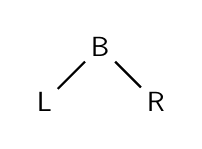
\begin{tikzpicture}
    \node (top) at (0,0) {$\mathsf{B}$};
    \node [below left  of=top] (left)  {$\mathsf{L}$};
    \node [below right of=top] (right) {$\mathsf{R}$};

    % Now draw the lines:
    \draw [thick, shorten <=-2pt, shorten >=-2pt] (top) -- (left);
    \draw [thick, shorten <=-2pt, shorten >=-2pt] (top) -- (right);
\end{tikzpicture}
\end{center}

What's interesting to note is that the points of $\mathsf{BCover}$ always have maxima with respect to specialization order. That means it's always possible to non-deterministically join points of $\mathsf{BCover}$ together.

Just as we found that the ``conjunction'' and ``disjunction'' operations of pairs of Coq propositions preserved having binary covers, we can define continuous maps representing conjunction and disjunction over the $\mathsf{BCover}$ space:
\begin{align*}
\cdot \wedge \cdot &: \mathsf{BCover} \times \mathsf{BCover} \to \mathsf{BCover}
\\ x \wedge y &\triangleq \mathsf{cases}(x, y)
\begin{cases}
\mathsf{Left}, \mathsf{Left}
 \qquad &\Rightarrow \qquad
 \mathsf{L}
\\
\mathsf{Right}, \_\_
 \qquad &\Rightarrow \qquad
 \mathsf{R}
\\
\_\_, \mathsf{Right}
 \qquad &\Rightarrow \qquad
 \mathsf{R}
\end{cases}
\\
\cdot \vee \cdot &: \mathsf{BCover} \times \mathsf{BCover} \to \mathsf{BCover}
\\ x \vee y &\triangleq \mathsf{cases}(x, y)
\begin{cases}
\mathsf{Left}, \_\_
 \qquad &\Rightarrow \qquad
 \mathsf{L}
\\
\_\_, \mathsf{Left}
 \qquad &\Rightarrow \qquad
 \mathsf{L}
\\
 \mathsf{Right}, \mathsf{Right}
 \qquad &\Rightarrow \qquad
 \mathsf{R}
\end{cases}.
\end{align*}

Are these definitions, using overlapping pattern matching, valid definitions? There are two conditions to check: that the cases cover the entire input space, and that overlapping branches have a maximum in terms of specialization order. Since the output space is $\mathsf{BCover}$, which always have maxima, we always satisfy the second condition. Since we have the cover
\[
\top_\mathsf{BCover} \le \mathsf{Left} \vee \mathsf{Right},
\]
we have in the product space
\begin{align*}
\top_{\mathsf{BCover} \times \mathsf{BCover}} \le 
  &(\mathsf{Left} \times \mathsf{Left}) \vee (\mathsf{Left} \times \mathsf{Right})
\\ \vee &(\mathsf{Right} \times \mathsf{Left}) \vee (\mathsf{Right} \times \mathsf{Right}),
\end{align*}
which clearly shows that the cases in the definitions of conjunction and disjunction also cover the entire input space.

It's still important to check that these definitions satisfy the definitions you'd expect for conjunction and disjunction on binary covers. Negation is easy as well:
\begin{align*}
 \neg &: \mathsf{BCover} \to \mathsf{BCover}
\\ \neg x &\triangleq \mathsf{cases}(x)
\begin{cases}
\mathsf{Left}
 \qquad &\Rightarrow \qquad
 \mathsf{R}
\\
\mathsf{Right}
 \qquad &\Rightarrow \qquad
 \mathsf{L}
\end{cases}
\end{align*}

\subsection{Alternative understandings of binary covers}

If you're bothered by the fact that the two opens in a binary cover get ``opposite'' treatments, and in particular that the logical operations on the second open are in reverse, for no good reason, there's another way to think about it. Rather than thinking of a binary cover of $A$ as two opens $P, Q : \Open{A}$ such that $A \subseteq P \cup Q$, we can instead think of it as an open set $P$ and a \emph{closed} set $\overline{Q}$ which is the ``set-theoretic'' complement of $Q$, since the complement of an open set is closed. Then the fact that $\langle P, Q \rangle$ is a binary cover means that $\overline{Q} \subseteq P$. Then the definitions of the logical operations should make more sense. For instance, one can find the union of two closed sets by taking their complement to produce two open sets, taking the intersection of that, and then taking the complement to return to a closed set. Since we are simply ``encoding'' closed sets with their open complements, computing the ``union'' just corresponds to taking an intersection.

This elicits the view of binary covers as ``approximate'' predicates, sandwiching a closed subspace inside an open one, with wiggle room for for points which are in between. Any points which are in $\overline{Q}$ (and thus also $P$) will definitely compute to $\mathsf{Left}$, while any points which are outside of $P$ (and thus also outside $\overline{Q}$) will definitely compute to $\mathsf{Right}$, while in-between points, which are in $P$ but not $\overline{Q}$, are allowed to compute either way.

Finally, note that there is a homeomorphism $\mathsf{BCover} \cong \PLower^+(\bool)$ given by
\begin{align*}
\mathsf{to} &: \mathsf{BCover} \to \PLower^+(\bool)
\\ \mathsf{to}(x) &\triangleq
  \mathsf{cases}(x)
  \begin{cases}
\mathsf{Left}
 \qquad &\Rightarrow \qquad
 \{ \mathsf{tt} \}
\\
\mathsf{Right}
 \qquad &\Rightarrow \qquad
 \{ \mathsf{ff} \}
  \end{cases}
\\
\mathsf{from} &: \PLower^+(\bool) \to \mathsf{BCover}
\\ \mathsf{from}(s) &\triangleq
  \mathsf{cases}(s)
  \begin{cases}
\lozenge(\cdot =\mathsf{tt})
 \qquad &\Rightarrow \qquad
 \mathsf{L}
\\
\lozenge(\cdot =\mathsf{ff})
 \qquad &\Rightarrow \qquad
 \mathsf{R}
  \end{cases},
\end{align*}
which gives another understanding of binary covers, as representing non-deterministic truth values in Boolean logic. All of the logical operations defined for binary covers might make more sense when interpreted by the homeomorphism above. For instance, the conjunction operation on Boolean values,
$\&\& : \bool \times \bool \to \bool$ can be lifted to a function of type $\PLower(\bool) \times \PLower(\bool) \to \PLower(\bool)$ which applies $\&\&$ to its non-deterministic input possibilities and collects all the possible results. This lifted $\&\&$ operation, when translated by the above homeomorphism to $\mathsf{BCover}$, identical to the $\wedge$ operation on $\mathsf{BCover}$s. This applies similarly to the other logical connectives that were defined on $\mathsf{BCover}$s.

This allows us to easily confirm that the logical connectives that we defined for $\mathsf{BCover}$s satisfy  De Morgan's laws for Boolean logic. In fact, binary covers form what is called a quasi-Boolean algebra, which satisfy almost all of the laws of Boolean algebra. Binary covers are similar to the three-valued logic K3, and also related to 

The specialization order on $\mathsf{BCover}$s corresponds to subset inclusion on $\PLower(\bool)$.

\subsection{Binary covers on $\R$}

The decidable predicates on a Coq type are analogous in \textbf{Top} to \emph{disconnections} or \emph{separations} of a space $A$, which are fancy terms for continuous maps $A \to \bool$ (just as decidable predicates on a type $A$ in Coq correspond to functions from $A$ to $\bool$). Equivalently, these are decompositions of a space into two disjoint opens. For the real numbers, $\R$, the only separation is the trivial one, where one open is the entire space, $\top_\R$, and the other the empty space, $\bot_\R$. When the only separations are trivial, in the case of $\R$, the space is called \emph{connected}, whose name accurately conveys the intuition of this notion for most spaces.

While there's a paucity of separations for $\R$, there is a wealth of binary covers, making it possible to ``do logic'', in a computable way (similarly as with decidable propositions), on $\R$. It's hard to exhaust all of them, but we can consider a particularly interesting class of them. For any tolerance $\varepsilon : \rat^+$, there is the map $\cdot <_\varepsilon \cdot : \R \times \R \to \mathsf{BCover}$ which satisfies for all $x, y : \R$
\begin{align*}
x <_\varepsilon y \models \mathsf{Left} 
\qquad &\Leftrightarrow \qquad
x < y
\\
x <_\varepsilon y \models \mathsf{Right} 
\qquad &\Leftrightarrow \qquad
x > y - \varepsilon,
\end{align*}
yielding an ``approximate'' comparison with error up to $\varepsilon$. Notice the intentional asymmetry in the definition here. We are setting up our our $\mathsf{BCovers}$ on $\R$ such that if an $\varepsilon$-approximate proposition ``computes'' that it lies in $\mathsf{Left}$, then it indeed lies in that open set indicated by the approximate proposition, while if it computes to $\mathsf{Right}$, it either doesn't lie in the indicated open, or it is ``barely inside'' the open, no more than $\varepsilon$ away from the border. However, this interpretation relies on never using the negation operator, since negation swaps these roles.

Just this $\R$-specific comparison operator is enough to reproduce all the logical operations of dReal, together with their computational meaning. dReal also offers a predicate $\cdot \le_\varepsilon \cdot$, which  is (computationally) identical to $\cdot <_\varepsilon \cdot$.
\footnote{This is due to the fact that, for any $x, y : \R$, the only way one could computationally/observationally confirm that $x \le y$ is by observing that $x < y$.}

\subsection{Compactness}

In the world of Coq, we observed if a predicate $P$ on a set $A$ is decidable and if $A$ is Kuratowski-finite, then $\forall a : A, P(a)$ and $\exists a : A, P(a)$ are decidable as well. The analog of this for \textbf{Top} are the compact/overt spaces.

[cite nLab]
A space $A$ is \emph{compact} if for every space $\Gamma$, and every open $U : \Open{\Gamma \times A}$, there is an open $\forall_A U : \Open{\Gamma}$ such that for every $V : \Open{\Gamma},$
\[
V \le_\Gamma \forall_A U \qquad \Leftrightarrow \qquad \top_A \times V \le_{\Gamma \times A} U.
\]
Similarly, a space $A$ is \emph{overt} if for every space $\Gamma$, and every open $U : \Open{\Gamma \times A}$, there is an open $\exists_A U : \Open{\Gamma}$ such that for every $V : \Open{\Gamma},$
\[
\exists_A U \le_\Gamma V  \qquad \Leftrightarrow \qquad U  \le_{\Gamma \times A} \top_A \times V.
\]

These conditions are the definitions of universal and existential quantification in terms of adjoints, viewing $\Gamma$ as some context and opens as truth values in a context.

A \emph{compact/overt} space is a space $A$ which is both compact and overt, as well as satisfying an additional property, that says for all $P, Q : \Open{A}$, we have
\[
\forall_A(P \vee Q) \le \forall_A P \vee \exists_A Q.
\]
I believe this additional requirement is equivalent to $A$ being closed (which is always true if $A$ is a subspace of a Hausdorff space, since every compact Hausdorff subspace is closed).
Now, suppose we have a compact/overt space $A$ which has opens $P, Q : \Open{A}$ which are a binary cover, i.e.,
\[
\top_A \le P \vee Q.
\]
To universally quantify over this binary cover, we'd like to show that
\[
\top_\Sigma \le \forall_A P \vee \exists_A Q,
\]
which follows from the derivation
\begin{align*}
\top_\Sigma 
  &\le \forall_A (\top_A)
\\ &\le \forall_A(P \vee Q)  \tag{since $\top_A \le P \vee Q$}
\\ &\le \forall_A P \vee \exists_A Q \tag{since $A$ is compact/overt}.
\end{align*}

Similarly, we can existentially quantify over the binary cover composed of $P, Q : \Open{A}$ to produce the binary cover
\[
\top_\Sigma \le \exists_A P \vee \forall_A Q,
\]
in a completely symmetric manner.

If we expand to work in the gros topos, where we have higher order functions, these functions for quantification, which allow us to extend quantification over opens to quantification over $\mathsf{BCover}$s, give us the operations $\forall_A : (A \to \mathsf{BCover}) \to \mathsf{BCover}$ and $\exists_A : (A \to \mathsf{BCover}) \to \mathsf{BCover}$ if $A$ is compact/overt.\footnote{Note that if $A$ is only compact or only overt, neither are possible, since the ``opposite'' quantification is used on the ``right'' side.}

Compact and overt subspaces of a space are closed under finitary union and intersection, so compact/overt subspaces are also closed under finite union and intersection. Additionally, the continuous image of a compact space is compact (just as the image of a finite space is finite), and likewise for overt spaces, so the continuous image of a compact/overt space is compact/overt.

For the real numbers, we have that for any real numbers $a, b : \R$ such that $a < b$, the closed interval from $a$ to $b$ is compact/overt. Of course, we can then take unions and intersections of intervals and still have compact/overt subspaces. This corresponds to the fact that dReal is able to quantify over intervals of $\R$.

\subsection{Non-determinism}

The generalization of decidable propositions to binary covers, and of finite sets to compact/overt spaces, should give us hope that exhaustive reasoning over continuous spaces is possible in many real-world scenarios, in particular because there ought to be plenty of useful binary covers and compact/overt spaces for verification tasks. The fact that the continuous image of a compact/overt space is compact/overt means that, as long as the space of inputs is compact/overt, and the query about the outputs is a binary cover, it is possible to just compute an answer to the query.

However, there's an issue with this line of argument, which is that continuous systems often make discrete decisions over continuous spaces. In order to do this, their decisions are necessarily non-deterministic. What this means is that rather than the output being some space $A$, which we might imagine to be a nice space, it is $\PLower(A)$, the space of overt subspaces of $A$. Since overt subspaces are not (in general) compact, we cannot simply quantify over $\PLower(A)$, even though this is what we'd like to do. For instance, we might want to know whether our autonomous car stays in our ``safe region'' for every non-deterministic choice it might make, or whether it is close to leaving that ``safe region'' in any non-deterministic choice it might make.

This issue is quite fundamental. Let's consider a simple example of how significant it is to change the output space from $A$ to $\PLower(A)$. Let's consider functions from the closed unit interval $[0,1]$ to $\R$. Any continuous map $f : [0,1] \to \R$ must be bounded, since the continuous image of a compact space is compact. Intuitively, there's no room for the graph of $f$ to ``escape'' and do anything weird:

\begin{center}
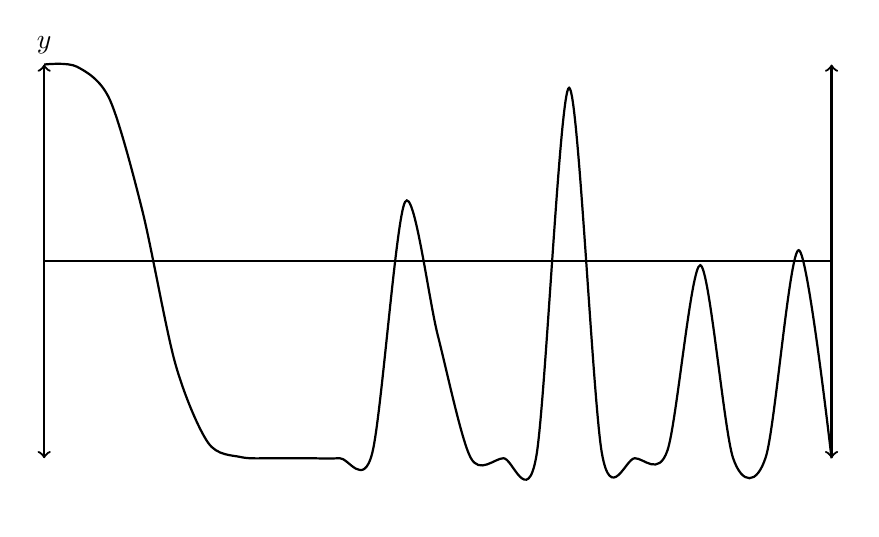
\begin{tikzpicture}[scale=2.5]
\draw[thick] (0,0) -- (4,0) node[right] {};
\draw[<->, thick] (0,-1) -- (0,1) node[above] {$y$};
\draw[<->, thick] (4,-1) -- (4,1);
\draw[scale=1,domain=0:4,smooth,thick,variable=\x] plot ({\x},{2*exp(-10*(sin(50*\x*\x))^2)-1});
\end{tikzpicture}
\end{center}

However, as soon as we allow non-determinism, we can do funky things. Here's a map $f : [0,1] \to \PLower(\R)$ which always maps each input to at most two outputs. Still, we see that $f$ no longer need be bounded:
\begin{center}
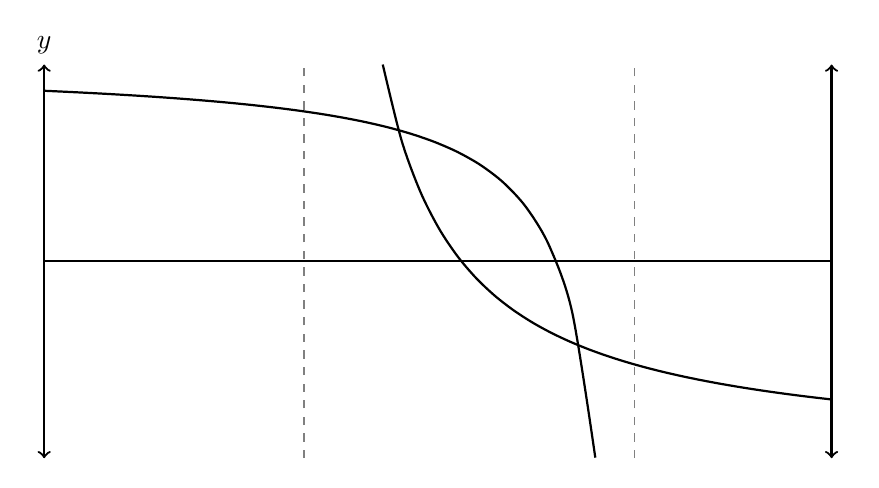
\begin{tikzpicture}[scale=2.5]
\draw[thick] (0,0) -- (4,0) node[right] {};
\draw[<->, thick] (0,-1) -- (0,1) node[above] {$y$};
\draw[<->, thick] (4,-1) -- (4,1);
\draw[scale=1,domain=0:2.8,smooth,thick,variable=\x] plot ({\x},{1 + 0.1/(0.25*(\x - 2) - 0.25))});
\draw[dashed, gray] (3,-1) -- (3,1);
\draw[scale=1,domain=1.72:4,smooth,thick,variable=\x] plot ({\x},{-1 + 0.2/(0.25*(\x - 2) + 0.17))});
\draw[dashed, gray] (1.32,-1) -- (1.32,1);
\end{tikzpicture}
\end{center}

Even though this is constructed from a non-deterministic merge of two deterministic cases, its behavior is potentially unbounded, because each of those cases is defined on an open subspace which in this case is not compact.

Another way in which nondeterminism can break compactness is by having a non-deterministic merging of infinitely many compact sets. For instance, consider
\begin{align*}
f &: [0,1] \to \PLower(\R)
\\ f(x) &\triangleq \mathsf{cases}(x)
\begin{cases}
[n : \nat] \quad &\cdot > 1 / (n + 1)
 \qquad \Rightarrow \qquad
 \{ n \}
\\ \quad &\cdot < 1/2
\qquad \qquad \ \  \Rightarrow \qquad
\{ 0 \}
\end{cases}
\end{align*}

When \emph{can} we admit exhaustive reasoning, then, for continuous maps of the form $A \to \PLower(B)$, where $A$ is compact? The first issue was that maps defined on an open space might not be bounded. One possible solution to this is to demand that each branch of a $\mathsf{cases}$ expression admit a continuous extension to a compact space. That is, suppose one of the branches is of the form $f : U \to \mathcal{P}(B)$, where $U$ is open and $\mathcal{P}(B)$ represents the space of compact/overt subspaces of $B$. Then $f$ admits a continuous extension to a compact space if there is some space $C$ which is compact/overt together with maps $i : U \to C$ and $g : C \to \mathcal{P}(B)$ such that $f = g \circ i$. Then, we have that $g(C) : \mathcal{P}(B)$ is compact/overt, and also that $f(U) \subseteq g(C)$, which means that we can \emph{soundly} reason about $f(U)$ by instead reasoning about $g(C)$. However, since $g(C)$ is in general larger than $f(U)$, it might not be the ``tightest'' reasoning that's possible.

For example, consider one of the branches of the map depicted above, which has the vertical asymptote. One of them is defined on the domain $(1/3, 1]$, which is not compact, and so it ``escapes'' off to $+\infty$ as it nears 1/3. This means that it will \emph{not} admit any continuous extension, as long as the codomain is kept as $\R$. By requiring that the branches of a $\mathsf{cases}$ expression admit continuous extensions to compact spaces, it prevents this kind of behavior. If the branch didn't have a vertical asymptote, we'd be able to extend it to the domain $[1/3, 1]$ which is compact/overt. We'd also be able to extend it to $[0,1]$ as well, in which case there would be many possible continuous extensions, and we could essentially make it behave as we wish in the region near 0. When we then analyzed the original branch, which was only on $(1/3, 1]$, the analysis wouldn't be as good, because of the garbage that we added in the new region.

A second issue was shown with the other map $f : [0,1] \to \PLower(\R)$, which had infinitely many branches. Even though each branch, evaluated at a single input point, was a compact/overt space, the union over the infinitely many branches, which sometimes all overlapped at once, was not necessarily compact. In this case, we had that $f(0) = \nat$, which is not compact in $\R$. A simple ``fix'' for this issue is to require having only finitely many branches.

These two conditions allow us to do some (incomplete) exhaustive reasoning about maps of the form $f : A \to \PLower(B)$, with $A$ compact/overt, which are defined by overlapping pattern matching. Here's the most general form in which I can phrase it. Suppose that $f$ is defined as
\begin{align*}
f &: A \to \PLower(B)
\\
f(x) &\triangleq \mathsf{cases}(x)
\begin{cases}
[i : I] \quad f_i(x) \qquad \Rightarrow \qquad \mathsf{inj}_{\lozenge}(e_i(x))
\end{cases},
\end{align*}
where $\mathsf{inj}_\lozenge : \mathcal{P}(B) \hookto \PLower(B)$ is the subspace inclusion which ``forgets'' compactness, the index set $I : \Type$ is finite, each $f_i : U_i \hookto A$ is an open embedding, and each $e_i : U_i \to \mathcal{P}(B)$ admits a continuous extension $e_i' : C_i \to \mathcal{P}(B)$ where $C_i$ is compact.

We wish that $f(A)$ were a compact/overt space such that we could reason about it, but in general, we only have that $f(A)$ is overt. However, we have that
\[
f(A) \subseteq \bigcup_{i : I} e_i'(C_i).
\]
Note that each $e_i'(C_i)$ is a compact/overt space: since the continuous image of a compact set is compact, we have $e_i'(C_i) : \mathcal{P}(\mathcal{P}(B))$, and by the monadicity of $\mathcal{P}$, we can also consider it as just $\mathcal{P}(B)$. Therefore, the union on the right-hand side is a finite union of compact/overt subspaces of $B$, and so it is also compact/overt. Define $C \triangleq \bigcup_{i : I} e_i'(C_i)$. We can exhaustively reason over $C$ with $\mathsf{BCover}$-valued predicates on $B$. If we have $P : B \to \mathsf{BCover}$, and we find that
\[
\forall_C P \models \mathsf{Left},
\]
then certainly $P^{-1}(\mathsf{Left})$ holds everywhere in $f(A)$. Similarly, if we find that
\[
\exists_C P \models \mathsf{Right},
\]
then certainly $P^{-1}(\mathsf{Right})$ holds everywhere in $f(A)$.

%\section{Computing with random samples with probability 1}
%\newcommand{\Stream}{\mathsf{Stream}}
\newcommand{\Prob}{\mathcal{R}}

\subsection{Introduction}

Suppose we have access to a random bitstream which affords us an ``API'' to access it, $s \leftarrow \mu_R$, where $\mu_R : \Prob(\Stream(\bool))$ is the probability distribution over bitstreams which gives equal probability to all bitstreams, and where we can think of $\Stream$s as being coinductively defined to in some sense ``prefer'' access to the front, but anyway we have the homeomorphism $\Stream(A) \cong \nat \Rightarrow A$, where $\Rightarrow : \Type \to \Space \to \Space$ constructs function spaces with discrete domains.

Now, suppose that I have real number in the unit interval with the binary expansion
\[
0. p_0\ p_1\ p_2\ \ldots,
\]
such that we can think of $p : \Stream(\bool)$ as well. I want to sample a Boolean value which is true with probability $p$. We can write the following recursive map which compares streams of Boolean values:
\begin{align*}
\mathsf{cmp} &: \Stream(\bool) \times \Stream(\bool) \to \bool_\bot
\\ \mathsf{cmp}(x, y) &\triangleq \mathsf{cases}(x, y)
\begin{cases}
b_x :: x'\ ,\ b_y :: y'
\quad \Longrightarrow \quad
\mathsf{cases}(b_x, b_y)
  \begin{cases}
  \mathsf{true}\ ,\ \mathsf{false} \quad &\Longrightarrow \quad
    \mathsf{strict}(\mathsf{false})
    \\
    \mathsf{false}\ ,\ \mathsf{true} \quad &\Longrightarrow \quad
    \mathsf{strict}(\mathsf{true})
    \\
    \mathsf{false}\ ,\ \mathsf{false} \quad &\Longrightarrow \quad
    \mathsf{cmp}(x', y')
    \\
    \mathsf{true}\ ,\ \mathsf{true} \quad &\Longrightarrow \quad
    \mathsf{cmp}(x', y')
  \end{cases}
\end{cases}
\end{align*}

Then, to use our random bitstream $s$ to return a Boolean value which is true with probability $p$, we need only compute the comparison $\mathsf{cmp}(p, s) : \bool_\bot$. The issue, which is indicated by the return type of this comparison, is that the comparison doesn't necessarily terminate. What if it happens to be that $p = s$? Then we are in a rut.

Fortunately, this \emph{isn't} the case. While, in our situation, $p : \Stream(\bool)$ is a point of the space, $s \leftarrow \mu_R$ is \emph{not} a point. That's because $\mu_R$ is non-atomic, which means that for any \emph{global point} $p$ of $\Stream(\bool)$,
\[
\mu_R(\cdot \neq p) = \mu_R(\top) = 1.
\]
That is, for any point $p$, $s$ is \emph{not} $p$ (with probability 1).

\cite{simpson2012} defines the ``locale of random sequences'' for a given measure $\mu$, which satisfy all measure-1 properties of that measure. By the previous reasoning, these spaces must not have any points. However, they still have computational structure, and I would like to tentatively argue in this note, that we can avoid dealing with reasoning about termination of functions like $\mathsf{cmp}$ defined on $\Stream(\bool)$ by using that structure. Instead of dealing with $\Stream(\bool)$, we use a subspace of it, called $\Stream(\bool)_{\mu_R}$, which is defined by the nucleus [refer to nLab for definition]
\[
U \mapsto \bigcup \left\{ V \suchthat U \subseteq V, \mu_R(U) = \mu_R(V) \right\},
\]
so that instead we would have for every \emph{global} point $p : \Stream(\bool)$,
\footnote{There are likely predicativity issues here, since there are more and more such global points as you increase the universe level of the ``predicative locale'' which these are points of. This is likely related to the predicativity issues of the double negation sublocale.}
\[
\mathsf{cmp}_p : \Stream(\bool)_{\mu_R} \to \bool.
\]
This in fact defines a valid nucleus. It wasn't clear to me that it preserves meets, so I emailed Antonin, and he provided a very nice explanation why it does in fact preserve meets.
\footnote{Why can't you have 
\[
\mathsf{cmp} :  \Stream(\bool) \times \Stream(\bool)_{\mu_R} \to \bool?
\]
Well, we have the mono $i_{\mu_R} : \Stream(\bool)_{\mu_R} \rightarrowtail \Stream(\bool)$, and imagining $s \leftarrow \mu_R$, we could then compute
\[
\mathsf{cmp}(i_{\mu_R}(s), s),
\]
which we know never terminates. The fact has to be that one input should be a global point, and the other must be random from a non-atomic probability distribution.}

Writing this program seems pointless, because as it turns out, the space $\Stream(\bool)_{\mu_R}$ doesn't have any points, since $\mu_R$ is non-atomic. So it seems like we can't ever run $\mathsf{cmp}$. But this isn't really the case: the random stream $s \leftarrow \mu_R$, which is perhaps pulling from \texttt{/dev/random}, while certainly not a \emph{point} of $\Stream(\bool)_{\mu_R}$ (after all, this space has no points), implements the (seemingly-impossible) computational \emph{interface} for $\Stream(\bool)_{\mu_R}$.

At least, it does so with probability 1. My point is that using doubly-negated spaces and probability distributions over them, gives a useful formalism for not having to reason about probability 1 termination. All of capacity for non-termination is localized in the ``API'' interface for the random stream $s \leftarrow \mu_R$. In $\Stream(\bool)_{\mu_R}$, we have the cover
\[
\top_{\Stream(\bool)_{\mu_R}} \subseteq
  \bigcup_{n : \nat} [n \mapsto \mathsf{true}],
\]
which in English says that every $\Stream(\bool)$ drawn from $\mu_R$ eventually has a $\mathsf{true}$ somewhere in its sequence. This is of course missing the stream which is always $\mathsf{false}$, but that's all its missing, and because it occurs with probability 0 under $\mu_R$ we can neglect it.

The above cover has an obvious computational interpretation, let's say for our random stream $s \leftarrow \mu_R$. We must be able to \emph{compute} some index $n$ such that the $n$th element is $\mathsf{true}$. This might take a long time, potentially, but with probability 1, it is finite.

There's some philosophical question to be asked: certainly my random stream is \emph{some} stream, so if I happened to write a program that compares the random stream with another stream which happens to be the same exact one. And then it wouldn't terminate. But if we're waiting a long time, it could just be that we're impatient, and we need to wait longer. So even if you did manage to miraculously ``hit some probability 0 event'' in some sense, there's no way to be sure.

\subsection{Reestablishing decidability}

When I tell people that all functions in \contpl{} must be continuous, they get worried. They fret that they can't write a step function, or make a decision over a continuous variable. It may seem particularly worrying when it comes to dealing with probability, where it is only possible to compute the probability of an event if the event is decidable (i.e., clopen). On $\R$, there are no non-trivial open sets, so it seems that computing with probability distributions on $\R$ is a lost cause, if one can't compute the probability of any nontrivial event.

Computing these probabilities is hard for a reason. Suppose we have a distribution $\mu : \Prob(\R)$ and want to compute the probability of the open predicate $\cdot > 0$. The probability $\mu(\cdot > 0)$ is a lower real number, since $\cdot > 0$ is open, which is not useful for computation. It is necessarily hard to upper-bound $\mu(\cdot > 0)$. Suppose that $\mu = \delta(x)$, the Dirac delta distribution which has all its mass at a point $x$. Then $\mu(\cdot > 0) = 1$ if and only if $x > 0$, which is a Sierp\'inski-valued proposition, meaning that it is affirmable, but not refutable. To compute the measure of $\cdot > 0$ as a real number, we'd need to be able to compare $x$ with 0, which is not a computable (continuous) operation.

There are a few things we could do. Rather than attempting to compute the probability of an open set, we can compute the approximate probability of a binary cover of $\R$.\footnote{Binary covers are defined in another note.} Given a binary cover $(P, Q)$ of $\R$, that is, $P, Q : \Open{\R}$ and $\R \subseteq P \cup Q$, we can non-deterministically compute two real numbers, $x_P, x_Q : \R$ such that $x_P + x_Q = 1$ and $x_P \le \mu(P)$ and $x_Q \le \mu(Q)$. That is, we can split up the weight of $\mu$ into $P$ and $Q$, non-deterministically assigning any weight in $P \cap Q$ to either $x_P$ or $x_Q$.

For instance, for our predicate $\cdot > 0$, we might define a binary cover $(\cdot > 0)_\varepsilon : \R \to \mathsf{BCover}$ for any approximation tolerance $\varepsilon : \rat^+$, where
\begin{align*}
\mathsf{Left}^{-1}((\cdot > 0)_\varepsilon) &\triangleq \cdot > 0
\\ \mathsf{Right}^{-1}((\cdot > 0)_\varepsilon) &\triangleq \cdot < \varepsilon.
\end{align*}

Then, when we non-deterministically compute the probability of the $\mathsf{Left}$ and $\mathsf{Right}$ sides, the weight assigned to the $\mathsf{Left}$ side will be at most $\mu(\cdot > 0)$, the ``actual'' probability of the open $\cdot > 0$.

But this still seems unsatisfactory. If one cannot compute, \emph{exactly}, the probability that some normal distribution lies in an open interval (or \emph{any} non-trivial event), when there is clearly no theoretical obstacle to doing so, that would be a problem. There is a substantial difference between probability distributions such as Dirac deltas and normal distributions, and it is beneficial to treat them as two different objects.

Normal distributions are non-atomic, in the sense for any normal distribution $\mu$ and any \emph{global} point $p : \R$, $\mu(\cdot \neq p) = \mu(\top) = 1$. Therefore, normal distributions also give probability distributions over some subspace which has no points, which we'll call $\R_\mathcal{N}$. And while $\R_\mathcal{N}$ has no points, its space of probability distributions $\Prob\left(\R_\mathcal{N}\right)$ certainly does, since there is an obvious map of open sets $j_\mathcal{N} : \Open{\R} \to \Open{\R_\mathcal{N}}$ which is well-behaved and accordingly the map
\begin{align*}
j_\mathcal{N}^* &: \Prob\left(\R_\mathcal{N}\right) \to \Prob(\R)
\\ j_\mathcal{N}^*(\mu)(U) &\triangleq \mu(j_\mathcal{N}(U))
\end{align*}
is well-defined.

In $R_\mathcal{N}$, there is a wealth of decidable propositions (i.e., clopens), meaning that it is easy to compute the probability of many different events of $R_\mathbb{N}$. For instance, our predicate $\cdot > 0$ is now clopen! We have the cover
\[
\R_{\mathcal{N}} \subseteq (\cdot > 0) \cup (\cdot < 0),
\]
since for any normal distribution $\mu$,
\[
\mu\left((\cdot > 0) \cup (\cdot < 0)\right) = \mu(\R) = 1.
\]
Note that the covering for $\R_\mathcal{N}$ is non-trivial, even though $\R_\mathcal{N}$ has no points; even though I am using subset-like notation such as $\subseteq$ and $\cup$, these operations \emph{cannot} be interpreted as operations on subsets. Unlike sets, where all empty sets are isomorphic, two spaces without points are not necessarily homeomorphic to each other.

Since $\cdot > 0$ is clopen, this means that for any probability distribution $\mu : \Prob\left(\R_\mathcal{N}\right)$, we can compute the probabilities $\mu(\cdot > 0)$ and $\mu(\cdot < 0)$, and know that their sum is exactly 1. Many operations impossible on $\R$ are newly possible on $\R_\mathcal{N}$. 

We can compute floors with a pattern match with infinitely many cases:
\begin{align*}
\lfloor \cdot \rfloor &: \R_\mathcal{N} \to \nat
\\ \lfloor x \rfloor &\triangleq \mathsf{cases}(x)
\begin{cases}
[n : \nat] \quad n < \cdot < n + 1
  \qquad \Longrightarrow \qquad
  n
\end{cases}
\end{align*}
This pattern match is well-defined, since there is indeed the cover
\[
\R_\mathcal{N} \subseteq \bigcup_{n : \nat} (n < \cdot < n + 1),
\]
because we have that for any normal distribution $\mu$,
\[
\mu \left( \bigcup_{n : \nat} (n - 1 < \cdot < n + 1) \right) = \mu(\R) = 1.
\]

Continuous maps whose domains are $R_\mathcal{N}$ may not be able to run on points, but they can be useful in other ways: for instance, they can be integrated against certain probability distributions (distributions on $\R_\mathcal{N}$), or computed on samples from such distributions, which are not points but ``lawless sequences'' in some sense. Also, we are able to condition on decidable predicates (whose probability is more than 0): that is, given a space $A$ and probability distribution $\mu : \Prob(A)$, if $U : \Open{A}$ is clopen and satisfies $\mu(U) > 0$, then we can compute a probability distribution $\mu(\cdot \suchthat U) : \Prob(\{A \suchthat U \})$, whose measure is defined by the usual equation
\[
\mu(P \suchthat U) \triangleq \frac{1}{\mu(U)} \mu(P \cap U).
\]
We note that the right-hand side is indeed a lower real number, as it is required to be: since $\mu(U)$ is a real number greater than zero, so is $\frac{1}{\mu(U)}$, and $\mu(P \cap U)$ is a non-negative lower-real number, and multiplying a positive real number by a non-negative lower-real gives a non-negative lower real number.

Therefore, for instance, we could compute a conditional probability distribution of the standard normal distribution, given the observation $\cdot < 0$.

\subsection{Products}

How does producing measure-1 subspaces interact with products? Suppose I have have probability distributions $\mu_A : A_{\mu_A}$ and $\mu_B : B_{\mu_B}$. That is, both probability distributions are restricted to their smallest measure-1 subspace. There should be a continuous map, which I believe is mono,
\[f : (A \times B)_{\mu_A \otimes \mu_B} \to A_{\mu_A} \times B_{\mu_B}.\]
Does this map have a continuous inverse? That is, are these spaces homeomorphic?

\subsection{Predicativity worries}
All the statements which I'm making should be valid in an impredicative sense. But I'm worried about how to actually define the smallest measure-1 subspaces in a computational (predicative) way. For doubly-negated spaces, which are somewhat similar, I should cite some references which indicate that doubly-negated spaces \emph{cannot} be inductively generated formal topologies, at least in some cases I think.

The fact that I'm now fairly confident that I want to be able to have these measure-1 subspaces in \contpl{} means that I might need to reconsider using inductively generated formal topologies as \emph{the} main setting for everything.

\subsection{More...}

[[Partial samplers become total since they terminate with probability 1 - this is something that *really* bothers probabilistic semantics people, I should make this a key argument ]]

%\section{Continuous extensions from dense subspaces}
%It's a well-known fact of classical topology that continuous maps (onto
Hausdorff spaces) are entirely determined by their behavior on 
dense subspaces of the input domain. For instance, a continuous function 
$f : \mathbb{R} \to \mathbb{R}$ is entirely determined by its values 
on rational inputs (since $\mathbb{Q}$ is dense in $\mathbb{R}$).

This fact becomes \emph{much} more useful in pointfree topology, where there are
many more dense subspaces than in classical topology. Some dense subspaces 
might not even have any points. For instance, any probability distribution
$\mu : \mathcal{R}(A)$ over a space $A$ is entirely specified by its
restriction to the subspace $\text{Ran}(\mu)$, which is the smallest subspace
of $A$ that has probability 1 under $\mu$ \cite{simpson2012}.
If $\mu$ is a non-atomic measure,
then $\text{Ran}(\mu)$ doesn't have any points. Still, $\text{Ran}(\mu)$ will
be dense if the support of $\mu$ is all of $A$. For instance, if $\mu$ is
a normal distribution, then $\text{Ran}(\mu)$ will be dense but have no points.

Using these random subspaces can help to clean up classical probability theory.
For instance, in classical probability theory, disintegrations of a probability
distribution are only unique up to probability-1 subsets. Given a probability
distribution $\mu$ over a product space $A \times B$, let 
$\nu : \mathcal{R}(A)$ be its marginal distribution over $A$. Then 
$f : A \to \mathcal{R}(B)$ is a \emph{disintegration} of $\mu$ if
$$ \mu = \int \text{map}(\lambda y. (x, y), f(x)) d\nu(x). $$
Notice that $f$ isn't necessarily unique. Two disintegrations may differ on
any null sets. What this means is that a disintegration $f$ isn't 
guaranteed to provide actually useful information on all its arguments;
sometimes its results can be completely arbitrary. For instance, if $\nu$ is a
Dirac delta distribution on some point $a : A$, then $f$ can be arbitrary
on parts of $A$ which are away from $a$, so it would be silly to try to impute
meaning from $f$'s behavior away from $a$. This dilemma has been discussed
\cite{shan2016}.

Only by switching to pointfree topology can we solve the probability-1 dilemma.
We simply restrict $\mu : \mathcal{R}(A \times B)$ to 
$\mu' : \mathcal{R}(\text{Ran}(\nu) \times B)$, since $\text{Ran}(\nu)$ has
the special property that \emph{all} of its ``non-empty" parts have non-zero measure.
Therefore, disintegrations of $\mu'$ must in fact be unique.

Still, this might be disappointing if $\text{Ran}(\nu)$ has no points, as
sometimes we might be interested in inspecting the value of the disintegration
$f$ at points of the original space $A$. Therefore, we might be interested to
know when we can continuously extend $f : \text{Ran}(\nu) \to \mathcal{R}(B)$
to a map $g : A \to \mathcal{R}(B)$, and when must such an extension \emph{itself}
be unique?

This note focuses on the second question, giving it a slightly more general
phrasing. Given a function $f : S \to B$ from a subspace $S$ of $A$, when is
uniqueness guaranteed for continuous extensions $g : A \to B$? We will not
worry about existence for now.

We will show that if $S$ is dense in $A$ and if $B$ is Hausdorff, then
continuous extensions (if they exist) must be unique. Recall that $S$ is 
\emph{dense} iff the nucleus $j : \mathcal{O}(A) \to \mathcal{O}(A)$ that presents
it has $j(\bot) = \bot$. $B$ is \emph{Hausdorff} iff the diagonal relation on $B$
is closed.

Since $B$ is Hausdorff, there is an open subspace
$$ \beta = \{ b : B \ |\ g(b) \neq g'(b) \}, $$
and accordingly, its complement, the subspace of $B$ where $g$ and $g'$ agree,
is closed and is the equalizer $\text{eq}(g, g')$.

Every closed subspace is co-classified by an open set $V$ such that its nucleus
$j$ is defined by 
$$j(U) = U \cup V.$$

Since $g$ and $g'$ agree on the dense subspace $S$, it must be that $S$
is a subspace of $\text{eq}(g, g')$, meaning that $\text{eq}(g, g')$ is also
dense, so that its nucleus $j$ satisfies $j(\bot) = \bot$. But since
$\text{eq}(g, g')$ is also closed, it has $j(\bot) = \bot \cup V$ for some $V$,
and therefore it must be that $V = \bot$, meaning that $j$ is the identity,
and that in fact $\text{eq}(g, g')$ is the entire space $A$, which in
turn yields the desired result that $g$ and $g'$ agree everywhere.

Here is a quick counterexample to show why $B$ must be Hausdorff.
Suppose that both
$A$ and $B$ are the Sierp\'inski space $\Sigma$, and that the dense subspace
$S$ of $\Sigma$ is the one which includes only the $\text{true}$ point of
$\Sigma$ (the ``open" point). Then the function $f : S \to B$ which maps
$\text{true}$ to $\text{true}$ can be extended both the identity map as well
as the constant $\text{true}$ map, which are distinct, even
though both are continuous extensions of $f$.

To apply this to disintegration, it would be interesting to know when 
$\mathcal{R}(A)$ is Hausdorff for a given space $A$. If $A$ is overt
and discrete, then certainly $\mathcal{R}(A)$ is Hausdorff. Since $A$
is discrete, this means that for any open set $U : \mathcal{O}(A)$
and any distribution $\mu : \mathcal{R}(A)$, $\mu(U)$ is a real number
(rather than just a lower real number).
Then we can define
\begin{align*}
\cdot \neq \cdot &: \mathcal{R}(A) \times \mathcal{R}(A) \to \Sigma
\\ \mu \neq \nu &\triangleq \exists a : A, \mu(\{ a \}) \neq \nu(\{a \})
\end{align*}
which will be true if and only if $\mu$ and $\nu$ are distinct,
meaning that $\mathcal{R}(A)$ is Hausdorff.

But often $\mathcal{R}(A)$ will not be Hausdorff. Taking $A = \Sigma$,
we observe that $\mathcal{R}(\Sigma)$ is homeomorphic to the closed
subspace of the non-negative lower real numbers which are no greater
than 1, which is not Hausdorff.

\section{Serendipity vs. semi-decision: alternative visions of constructive topology}

There are many approaches to developing topology in a manner that is in some sense ``constructive'', with the names of some principal contributors to each:

\begin{itemize}
\item Locale theory (Johnstone, Vickers)
\item Formal topology (Sambin, Vickers, Maietti, Palmgren)
\hrule
\item Abstract stone duality (Taylor)
\item Synthetic topology (Escard\'o, Bauer) 
\item natural topology (Waaldijk)
\item computable topology / represented spaces (Weihrauch) 
\end{itemize}

I claim that we can classify each theory as following as characterizing ``openness'' either by \emph{serendipity} or by \emph{semi-decision}. Formal topology and locale theory characterize openness by serendipity, while in the rest, opens are semi-decidable properties.

In the serendipitous approaches,
\begin{itemize}
\item Opens are closed under either arbitrary (impredicative) or set-indexed (predicative) joins
\item Points of the Sierp\'inski space are propositions (impredicative) or types (predicative). Two propositions (types) $U$ and $V$ are considered equal as points of the Sierp\'inski space if there are implications (constructions) $U \to V$ and $V \to U$.
\item Spaces without points may have non-trivial structure; two spaces which each have no points are not necessarily homeomorphic.
\end{itemize}

On the other hand, when opens are characterized as semi-deciders,
\begin{itemize}
\item Opens are closed under countable (internal view) or recursively enumerated (external view) joins
\item Points of the Sierp\'inski space are sequences $\nat \to \bool$, where a sequence is the ``true'' point if it has a $\mathsf{true}$ in it, and is false if it is is the constant sequence of all $\mathsf{false}$s.
\item Any two spaces which have no points are homeomorphic.
\end{itemize}

The slogan \emph{serendipity} comes from Steve Vickers. Vickers used the term \emph{serendipity} to indicate this distinction from semi-decidability, saying one of the concepts characterizing ``observability'' is \cite{vickersGeoThDB}
\begin{quote}
\emph{serendipity}: one is told how to know in retrospect when one has observed something, but not any method that's guaranteed to result in the observation whenever possible.
\end{quote}

In another example, Vickers gives as an example of an observable property the existence of the Loch Ness monster, saying that
\begin{quote}
we can well imagine under what conditions we could know that the assertion is true. To be sure, this would take a lot of luck, serendipity or Divine Grace, but no particular effort -- in fact we can imagine others putting much time and resources into a vain attempt to repeat our observation.
\end{quote}

Synthetic topology and abstract stone duality appear to accommodate both views by only requiring that $\Sigma$ forms a \emph{dominance} such that $\nat$ is overt. Depending on the model of synthetic topology, it may be the case that in fact $\Sigma$ has no other truth values than those required to make $\nat$ overt, in which case it is [cite http://math.andrej.com/wp-content/uploads/2010/01/csms_in_synthtop.pdf].

The connection with proofs should be obvious. An observable property is one for which we can check (i.e., decide) whether a putative proof is in fact a valid proof. So any type or proposition in Coq corresponds informally to an observable property in this sense. Now, given any proposition for which proof checking is decidable, we can semi-decide whether the proposition in fact holds, by checking all possible proofs. This is the connection between serendipity and semi-decision. For instance, consider the ``or'' operation. In the ``serendipity'' view, we serendipitously hope that we fall into either of the two explicit cases of the overlapping pattern match (rather than the catch-all case, which of course we fall in to), and if we are so lucky to do so, then our output will also luckily fall into the smaller open of the Sierp\'inski space. In effect, what the $\mathsf{cases}$ definition tells us is when it suffices to have proved the disjunction. The semi-decision view, instead of considering criteria for satisfactory proof, works with semi-decision procedures for finding proofs themselves, and therefore, to find a proof of the disjunction, the two proof finders must be interleaved.

I happen to favor the \emph{serendipity} view, because one can always go from serendipity to semi-decision, but not the other way around, and also because (at least naive) use of the semi-decision approach could result in some very slow programs, whereas in the serendipity point of view, we are required to provide proofs in order for computation to proceed. This is more work (you might complain about writing proofs), but it means that the resulting code will be more efficient. [Explaining this with an example would be a good idea.]

Any point of the ``semi-decision'' Sierp\'inski space can be converted to one in the ``serendipity'' Sierp\'inski space, but not necessarily the other way around. However, from an external perspective, searching for proofs (or inhabitants of types) is semi-decidable, giving a sort of connection in the other direction. 

This distinction is a key difference between the formal topology approach and the Marshall language by Andrej Bauer and Paul Taylor, which takes the approach of semi-decision. This means that one needs not provide proofs of validity of definitions made in the language. Incorrect definitions either return inconsistent/incorrect results or fail to terminate. However, I imagine that the tradeoff is that programs can be slower than if the other approach were taken.


\bibliographystyle{alpha}
\bibliography{Main}

\end{document}
